% !TeX spellcheck = de_CH_frami

\section{Spectral Graph Wavelet Transformation\label{sec:sgwt:wavelets}}
\rhead{SGWT}

Hier wollen wir nun das Bisherige zur Spectral Graph Wavelet Transformation 
vereinen.

\subsection{Graph Fourier Transformation\label{subsec:sgwt:gft}}

Bevor wir uns auf die Graph Wavelets st\"urzen, wollen wir zuerst versuchen die 
Fourier Theorie auf Funktionen auf Graphen anzuwenden. Dazu nehmen wir das 
Beispiel eines Dirac-Stosses $\delta(x)$, siehe~\cref{fig:sgwt:fft:dirac}.
Wenn wir davon die Fourier Transformation berechnen, zu sehen 
in~\cref{fig:sgwt:fft:fftreal} und~\cref{fig:sgwt:fft:fftimag}, stellen wir 
fest, dass wir darin alle Frequenzen wiederfinden. Die Fouriertransformierte 
$\hat{\delta}$ ist somit vollst\"andig delokalisiert.
\begin{figure}
    \begin{minipage}[t]{\textwidth}
    \centering
    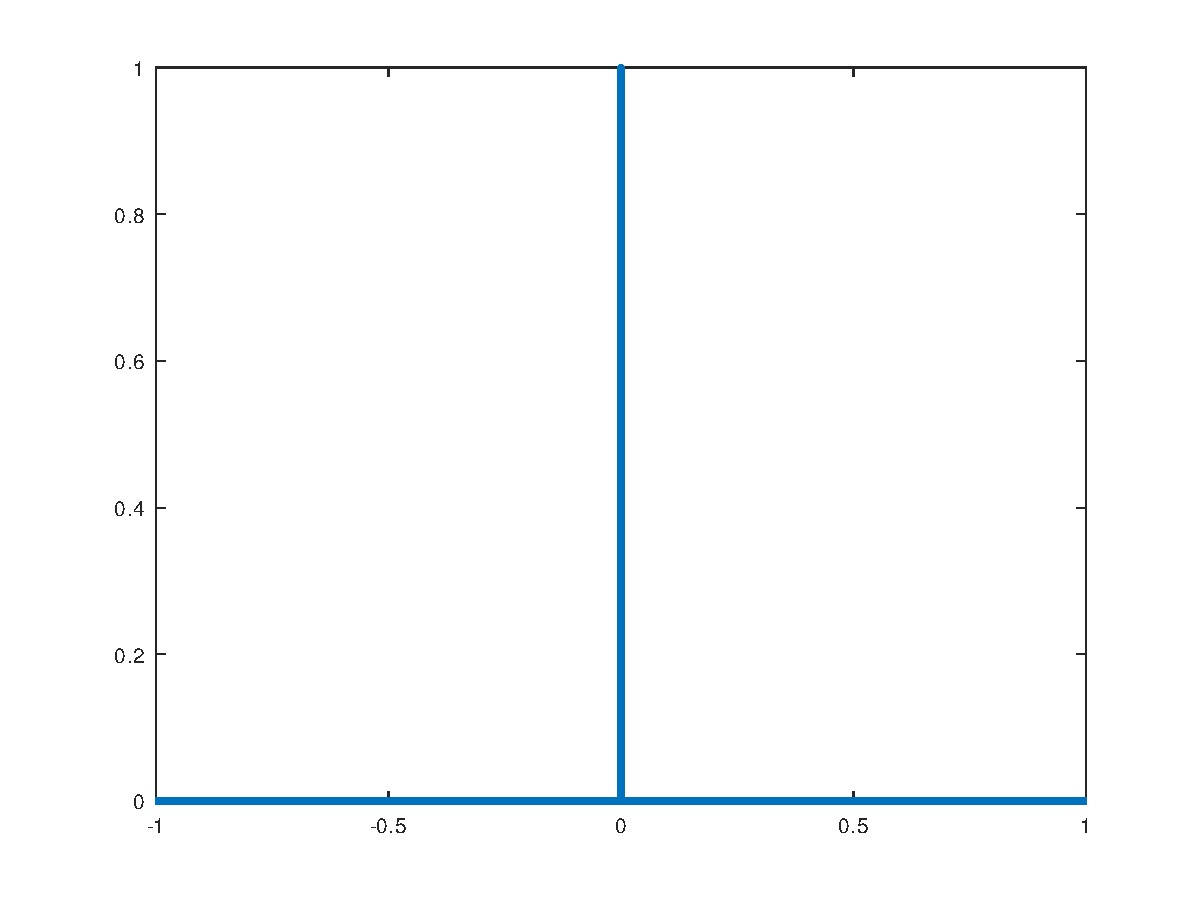
\includegraphics[
    width=0.7\textwidth
    ]{papers/sgwt/images/dirac/dirac_delta.pdf}
    \vspace{-10pt}
    \caption{Darstellung eines Dirac-Stoss $\delta(x)$ mit maximal Wert $1$. 
    \label{fig:sgwt:fft:dirac}}
    \end{minipage}
    ~
    \begin{minipage}[t]{0.49\textwidth}
    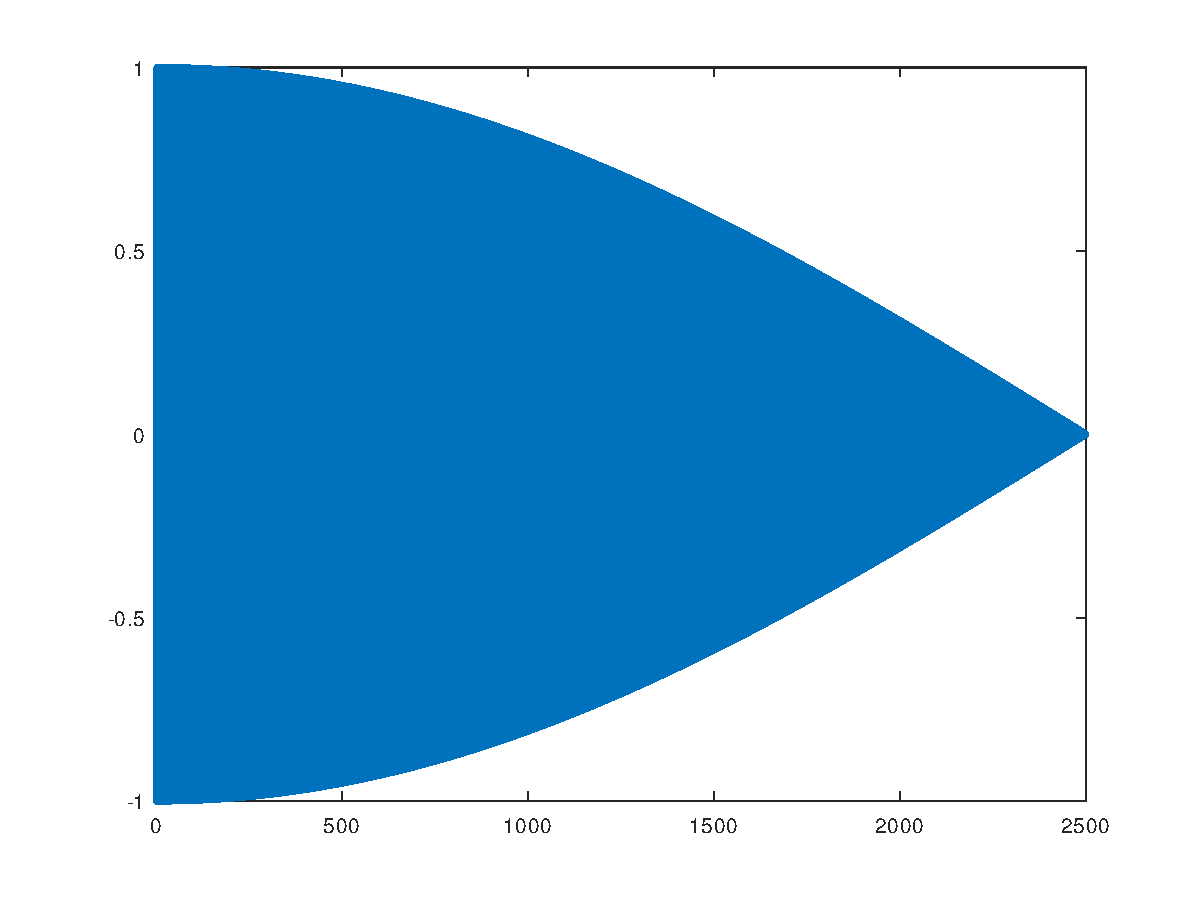
\includegraphics[
    width=\textwidth
    ]{papers/sgwt/images/dirac/dirac_fft_real.pdf}
    \vspace{-20pt}
    \caption{Kosinus Anteile $a_n$  der Fourier Transformation des 
    Dirac-Stosses $\hat{\delta}(x)$.
    \label{fig:sgwt:fft:fftreal}}
    \end{minipage}
    ~
    \begin{minipage}[t]{0.49\textwidth}
    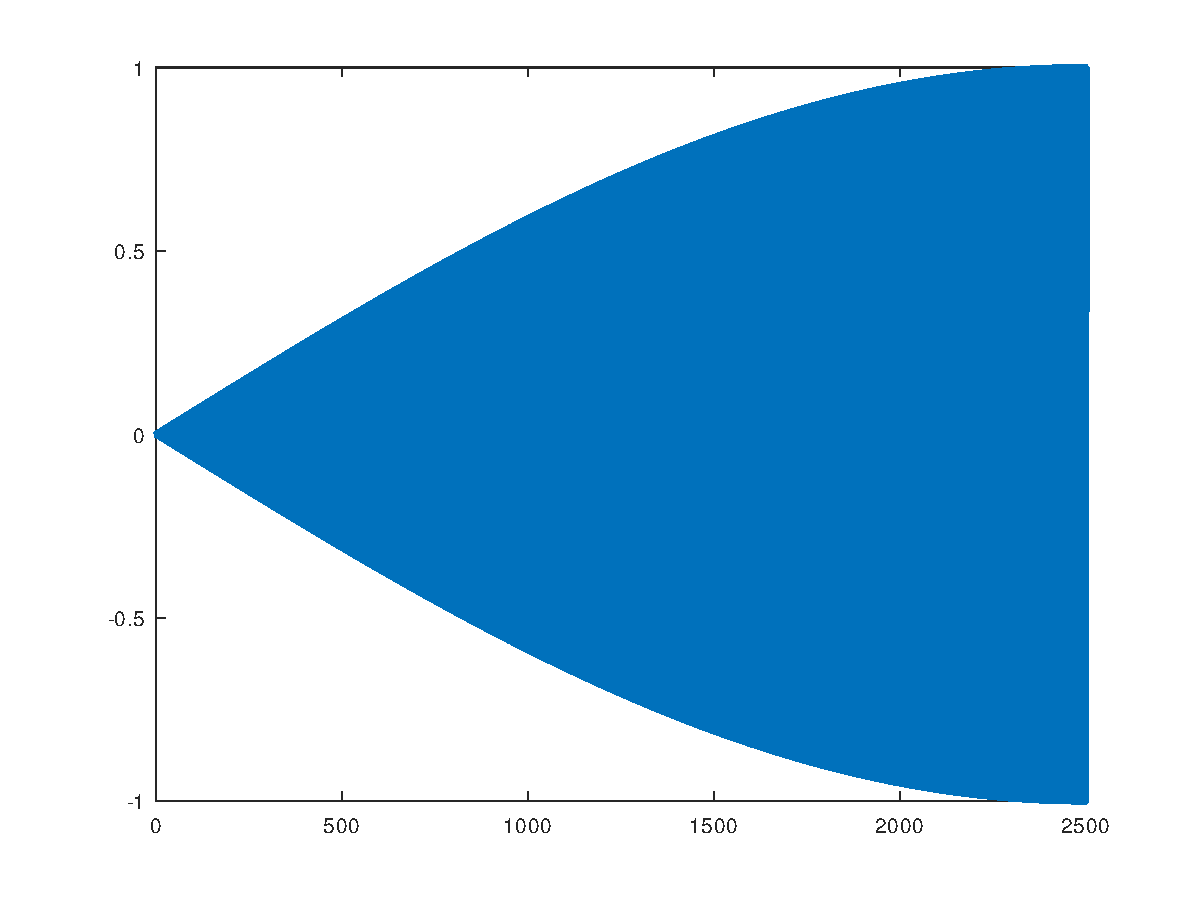
\includegraphics[
    width=\textwidth
    ]{papers/sgwt/images/dirac/dirac_fft_imag.pdf}
    \vspace{-20pt}
    \caption{Sinus Anteile $b_n$ der Fourier Transformation des Dirac-Stosses 
    $\hat{\delta}(x)$.
    \label{fig:sgwt:fft:fftimag}}
    \end{minipage}
\end{figure}

Mit den in ~\cref{sec:sgwt:spectralanalysis} vorgestellten Eigenfunktionen 
k\"onnen wir aber nutzen um eine Graph Fourier Transformation zu definieren. 
Dazu ersetzen wir bei der Fourier Transformation die Exponentialfunktion durch 
die Eigenvektoren der Laplace Matrix und erhalten
\begin{equation*}
\hat{f} = \langle \chi, f \rangle = \sum_{n = 1}^{N} \chi^*(n)f(n).
\end{equation*}
Wenn wir, wie zum Beispiel in \texttt{octave} \"ublich, die Eigenvektoren als 
Spalten einer Matrix
\begin{equation}
\chi = 
\left[
\begin{pmatrix}\\\chi_0\\\\\end{pmatrix}
\begin{pmatrix}\\\chi_1\\\\\end{pmatrix}
\begin{pmatrix}\\\chi_2\\\\\end{pmatrix}
\cdots
\begin{pmatrix}\\\chi_{N-1}\\\\\end{pmatrix}
\right]
\end{equation}
zur Verf\"ugung haben, k\"onnen wir die Transformation 
einfach durch eine Matrix-Vektor Multiplikation ersetzen
\begin{equation*}
\hat{f} = \chi^* f.
\end{equation*}
Die R\"ucktransformation ist dann auch wieder analog der Fouriertheorie
\begin{equation*}
f = \chi \hat{f}.
\end{equation*}

\subsection{Graph Wavelets: Lokalisierung\label{subsec:sgwt:gwt:localizing}}

Mit der Graph Fourier Transformation k\"onnen wir nun Funktionen auf Graphen 
analysieren und dann auch wieder synthetisieren, aber noch nicht zu 
lokalisieren. Wir m\"ussen also unsere Graph Fourier Transformation zur Graph 
Wavelet Transformation erweitern, denn diese erm\"oglichen uns, genau dies zu 
tun.

Leider haben Graphen den Nachteil, dass die Knoten keine inh\"arente 
Reihenfolge haben. Es ist also nicht klar was mit $f(v - h)$ gemeint ist. Wir 
haben allerdings in~\cref{eq:sgwt:lambda:series} eine Reihenfolge f\"ur die 
Eigenwerte der Laplace Matrix eines Graphen definiert. Die Eigenwerte sind 
allerdings vollst\"andig lokalisiert, womit sie einem Dirac-Stoss an einem 
Knoten gleich kommen. Wir k\"onnten also versuchen das Spektrum des Graphen so 
zu manipulieren, dass eine Lokalisierung m\"oglich wird.

Mit der Definition verschiedener Kernelfunktionen, wollen wir genau diese 
Lokalisierung im Spektrum erreichen. Wir konstruieren dazu eine Kernelfunktion 
$g(\lambda)$, welche die Eigenschaften $g(0) = 0$ und $\lim_{\lambda\to\infty} 
g(\lambda) = 0$ erf\"ullt. Mit Hilfe dieses Bandpasses k\"onnen wir die 
Eigenwerte bewusst lokalisieren.
Wir nehmen also wieder den Dirac-Stoss $\delta(v)$, 
siehe~\cref{fig:sgwt:gft:dirac}, und einen Ringgraphen, da dieser die normalen 
Fourier Transformation am besten 
approximiert. Darauf wenden wir jetzt die Graph Fourier Transformation an, 
indem wir $\delta(v)$ mit $\chi^*$ multiplizieren.
In~\cref{fig:sgwt:gft:gft} sehen wir das Resultat dieser Multiplikation als eine
eine Kombination von~\cref{fig:sgwt:fft:fftreal} 
und~\cref{fig:sgwt:fft:fftimag}. \Cref{fig:sgwt:gft:gft} zeigt auch, 
dass die Graph Fourier Transformation nicht perfekt sondern nur eine 
Approximation der Fourier Transformation ist. Wenn wir jetzt die Kernelfunktion 
$g(\lambda)$ auf unser $\hat{\delta}(v)$ anwenden, erhalten wir ein im gewissen 
Masse lokalisiertes Spektrum in~\cref{fig:sgwt:gft:ggft}. Dieses lokalisierte 
Spektrum k\"onnen wir jetzt R\"ucktransformieren und erhalten damit unser 
erstes Wavelet $\psi$, zu sehen in~\cref{fig:sgwt:gft:iggft}.
\begin{figure}
    \centering
    \begin{minipage}[t]{0.49\textwidth}
        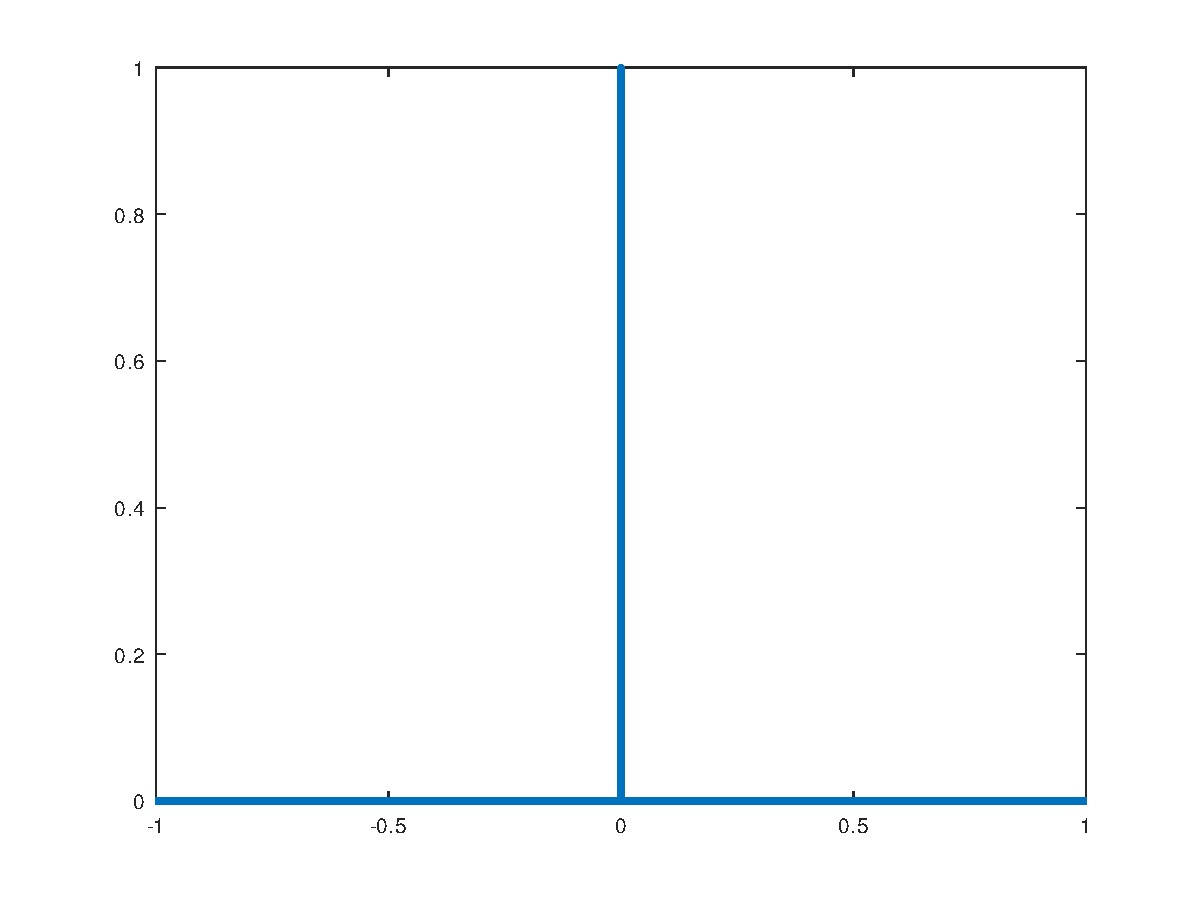
\includegraphics[
        width=\textwidth
        ]{papers/sgwt/images/dirac/dirac_delta.pdf}
        \vspace{-20pt}
        \caption{Darstellung eines Dirac-Stoss $\delta(v)$ mit maximal 
        Wert $1$. \label{fig:sgwt:gft:dirac}}
    \end{minipage}
    ~
    \begin{minipage}[t]{0.49\textwidth}
        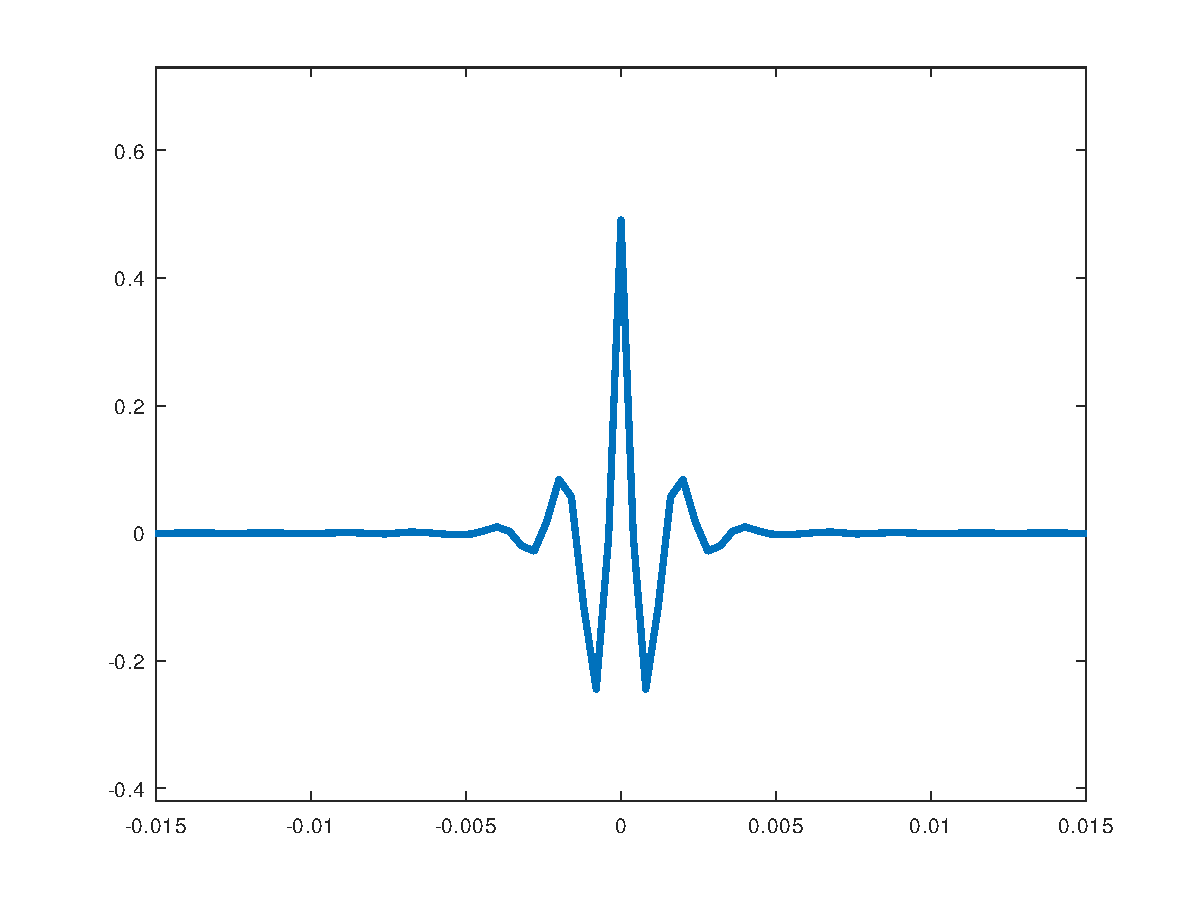
\includegraphics[
        width=\textwidth
        ]{papers/sgwt/images/dirac/dirac_g_igft.pdf}
        \vspace{-20pt}
        \caption{R\"ucktransformation der mittels Kernelfunktion $g(\lambda)$ 
            modifizierten Dirac-Stoss Graph-Transformation        
            aus~\cref{fig:sgwt:gft:ggft}, 
            $\psi = \chi\hat{\delta}_g(\lambda)$.
            \label{fig:sgwt:gft:iggft}}
    \end{minipage}
    ~
    \begin{minipage}[t]{0.49\textwidth}
        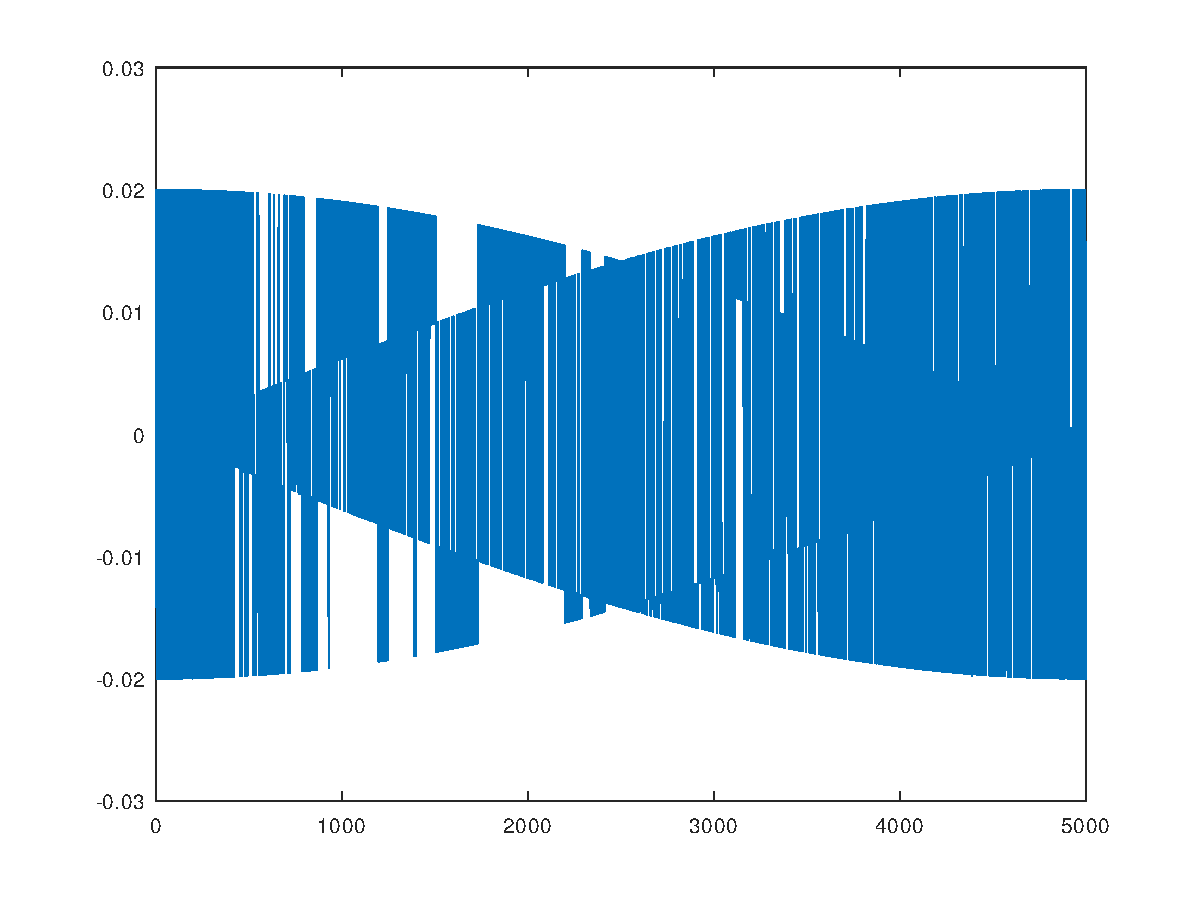
\includegraphics[
        width=\textwidth
        ]{papers/sgwt/images/dirac/dirac_gft.pdf}
        \vspace{-20pt}
        \caption{Graph-Transformation des Dirac-Stosses 
            aus~\cref{fig:sgwt:gft:dirac},
            $\hat{\delta}(v) = \chi^*\delta(v)$.
            \label{fig:sgwt:gft:gft}}
    \end{minipage}
    ~
    \begin{minipage}[t]{0.49\textwidth}
        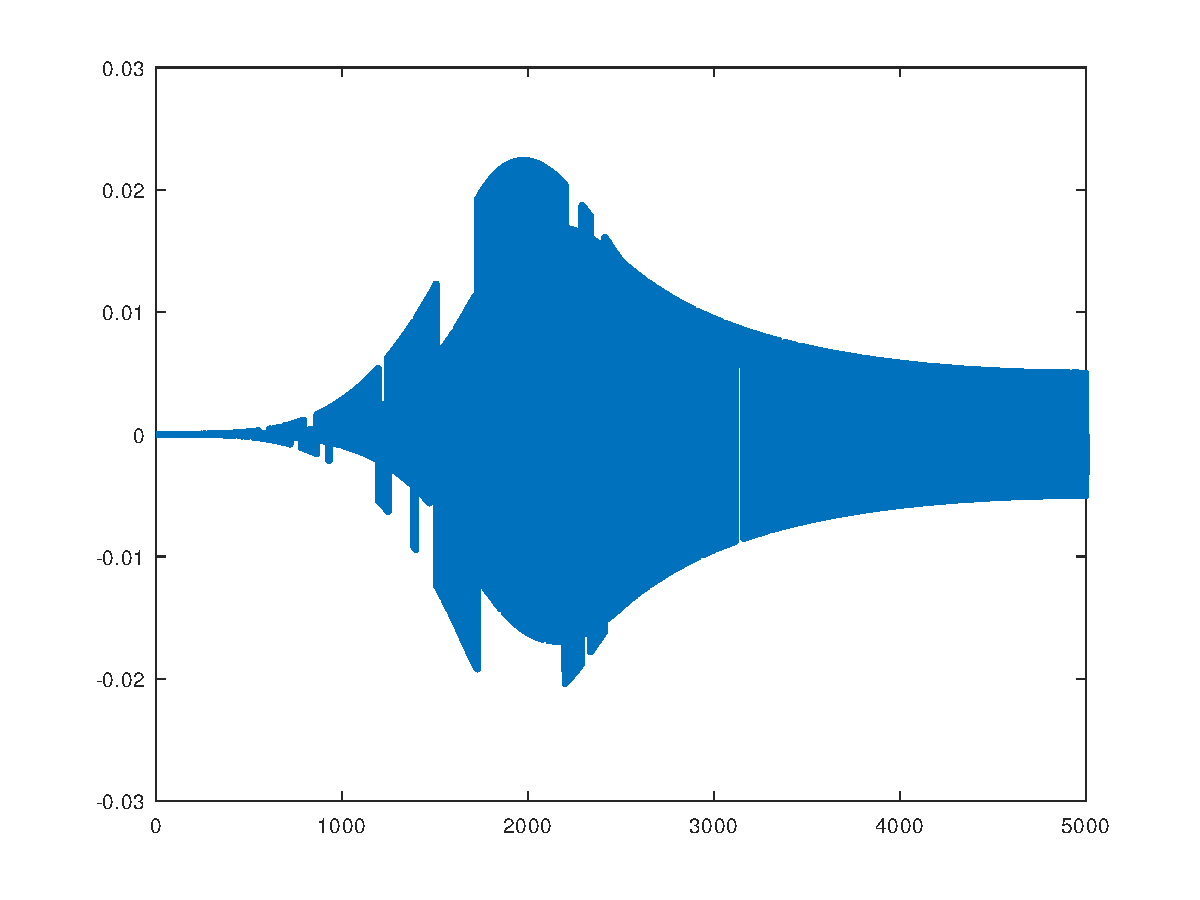
\includegraphics[
        width=\textwidth
        ]{papers/sgwt/images/dirac/dirac_g_gft.pdf}
        \vspace{-20pt}
        \caption{Anwendung der Kernelfunktion $g(\lambda)$ auf die Graph 
            Transformation des Dirac-Stosses $\hat{\delta}(v)$ 
            aus~\cref{fig:sgwt:gft:dirac},
            $\hat{\delta}_g(\lambda) = g(\lambda)\hat{\delta}(v)$.
            \label{fig:sgwt:gft:ggft}}
    \end{minipage}
\end{figure}

Wir haben jetzt aber noch das Problem, dass $\lambda_0 = 0$ gilt. Wir verlieren 
also den konstanten Anteil der zu analysierenden und synthetisierenden 
Funktion. Um das zu l\"osen ben\"otigen wir eine zus\"atzliche 
Kernelfunktion $h(\lambda)$ mit den Eigenschaften $h(0) > 0$ und 
$\lim_{\lambda\to\infty} h(\lambda) = 0$, oder anders ausgedr\"uckt, wir 
ben\"otigen einen Tiefpass.

Diese neu gefundene Funktion $h(\lambda)$ k\"onnen wir wieder auf die Graph 
Fourier Transformierte eines Dirac-Stosses anwenden und erhalten damit
$\hat{\delta}_h(\lambda)$, zu sehen in~\cref{fig:sgwt:gft:hgft}. Die 
R\"ucktransformation, zu sehen in~\cref{fig:sgwt:gft:ihgft}, liefert uns damit 
dann unser zweites Wavelet $\phi$.
\begin{figure}
    \begin{minipage}[t]{0.49\textwidth}
        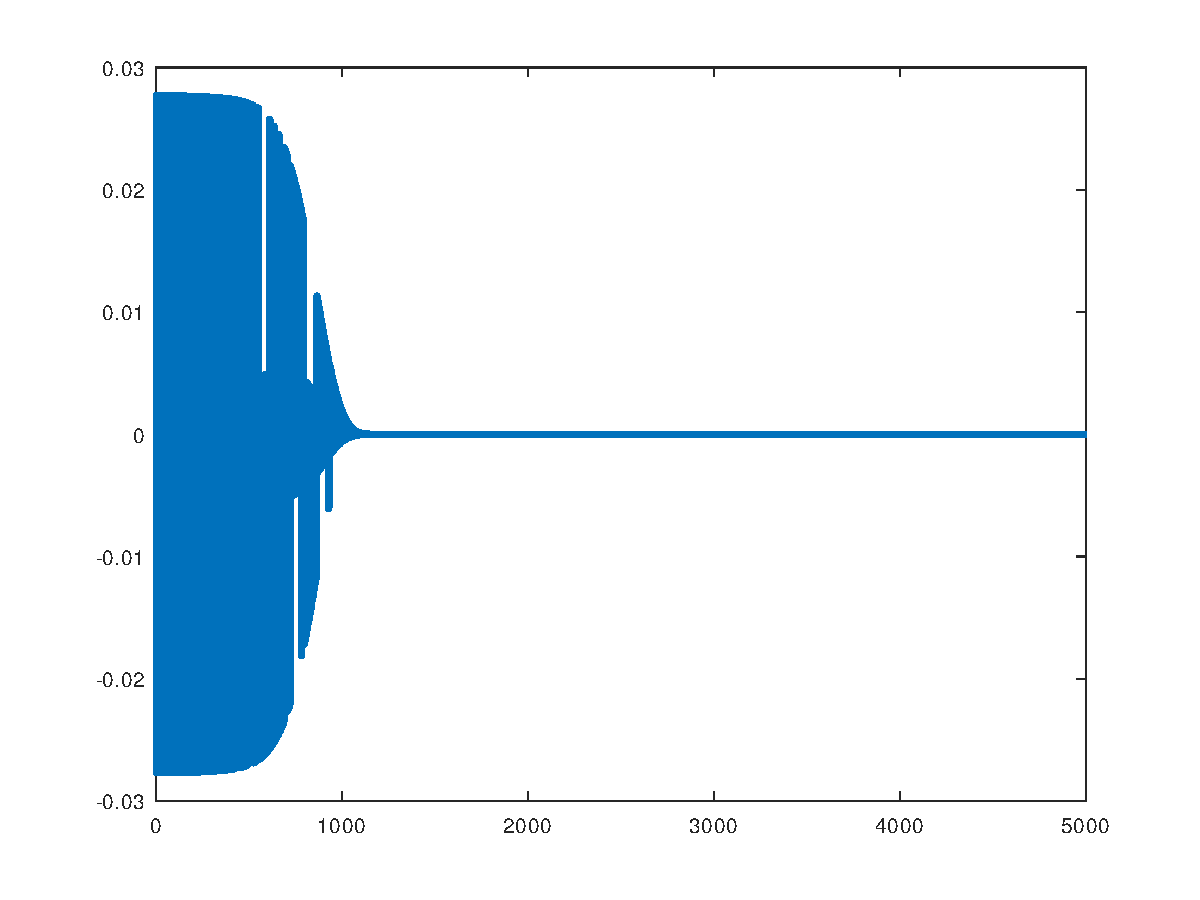
\includegraphics[
        width=\textwidth
        ]{papers/sgwt/images/dirac/dirac_h_gft.pdf}
        \vspace{-0pt}
        \caption{Anwendung der Kernelfunktion $h(\lambda)$ auf die Graph 
        Transformation des Dirac-Stosses $\hat{\delta}(v)$ 
        aus~\cref{fig:sgwt:gft:dirac}, $\hat{\delta}_h(\lambda) = 
        h(\lambda)\cdot\hat{\delta}(v)$.
        \label{fig:sgwt:gft:hgft}}
    \end{minipage}
    ~
    \begin{minipage}[t]{0.49\textwidth}
        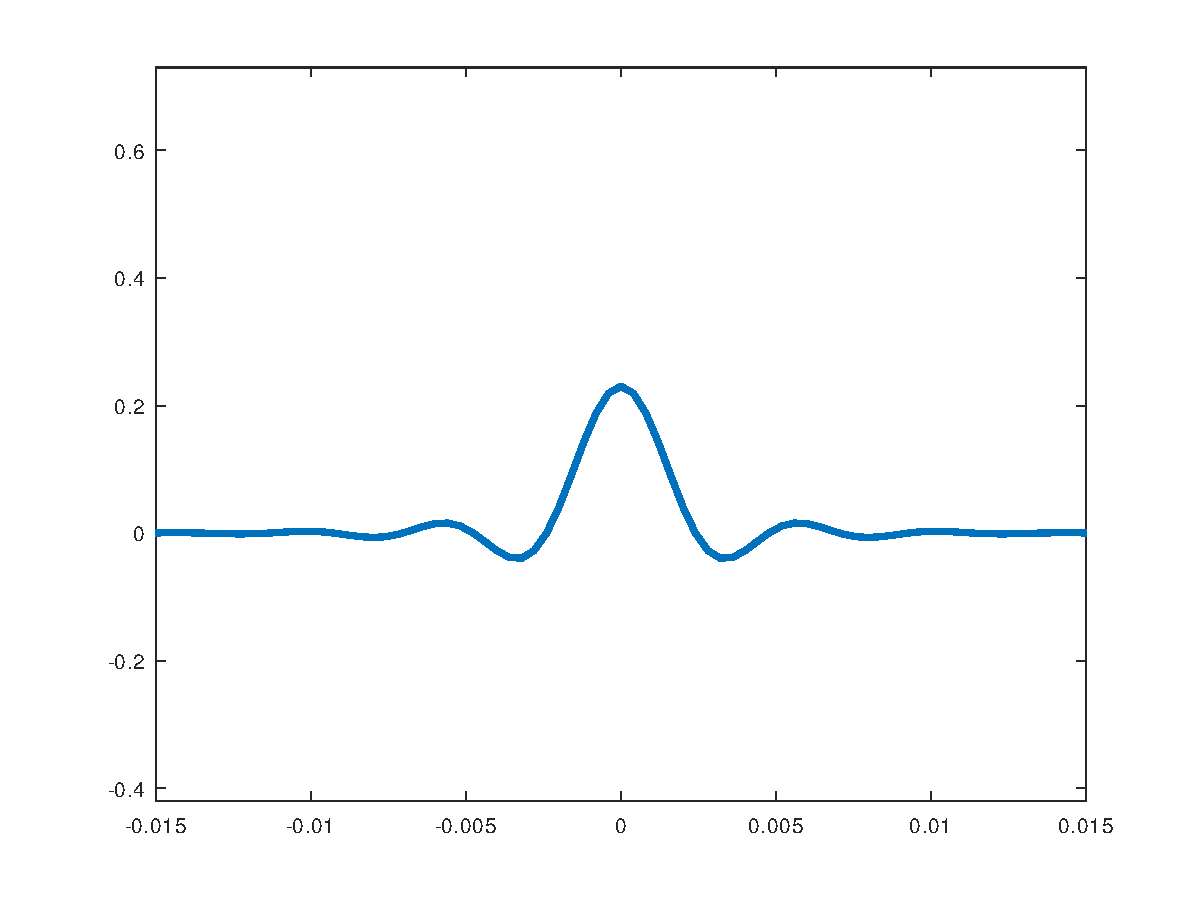
\includegraphics[
        width=\textwidth
        ]{papers/sgwt/images/dirac/dirac_h_igft.pdf}
        \vspace{-0pt}
        \caption{R\"ucktransformation der mittels Kernelfunktion $h(\lambda)$ 
        modifizierten Dirac-Stoss Graph-Transformation
        aus~\cref{fig:sgwt:gft:hgft}, $\phi = \chi\hat{\delta}_h(\lambda)$.
        \label{fig:sgwt:gft:ihgft}}
    \end{minipage}
\end{figure}

\subsection{Graph Wavelets: Skalierung\label{subsec:sgwt:gwt:scaling}}

Nachdem wir nun in~\cref{subsec:sgwt:gwt:localizing} eine M\"oglichkeit 
gefunden haben die Lokalisierung im Spektrum eines Graphen durchzuf\"uhren, 
fehlt uns noch ein Werkzeug zur Skalierung der Wavelets. Das Problem ist hier 
aber, dass ein Graph keine geometrische Skalierungstransformation kennt. Wir 
m\"ussen also versuchen, wie schon die Lokalisierung, unsere 
Skalierung im Spektrum des Graphen vorzunehmen. Dazu ben\"otigen wir einen 
Skalierungsfaktor $t$ den wir mit unseren Eigenwerten $\lambda$ multiplizieren.
Dabei wird verwendet, dass das Spektrum mit $D_a$ skaliertes klassischen 
Wavelet eben auch mit $D_{1/2}$ (modulo Normierungsfaktoren) skaliert. Statt 
dass wir also auf dem Graphen versuchen unser Wavelet zu skalieren, skalieren 
wir den Bandpass $g(\lambda)$, den wir ja auf das Spektrum anwenden und 
erhalten die Kernelfunktion $g(t\lambda)$. Dies ergibt dann eine skalierte 
Wavelet-Familie $\psi_t$.

\Cref{fig:sgwt:gft:gt1gft,fig:sgwt:gft:gt2gft,fig:sgwt:gft:gt3gft,fig:sgwt:gft:gt4gft,fig:sgwt:gft:gt5gft}
zeigen Beispiele von unterschiedlich skalierten Kernelfunktionen, 
die auf die Fourier Graph-Transformierte eines Dirac-Stosses angewandt werden.
\Cref{fig:sgwt:gft:igt1gft,fig:sgwt:gft:igt2gft,fig:sgwt:gft:igt3gft,fig:sgwt:gft:igt4gft,fig:sgwt:gft:igt5gft}
wiederum zeigen die daraus resultierende Wavelet-Familie $\psi_t$.
\begin{figure}
    \centering
    \begin{minipage}[t]{0.49\textwidth}
        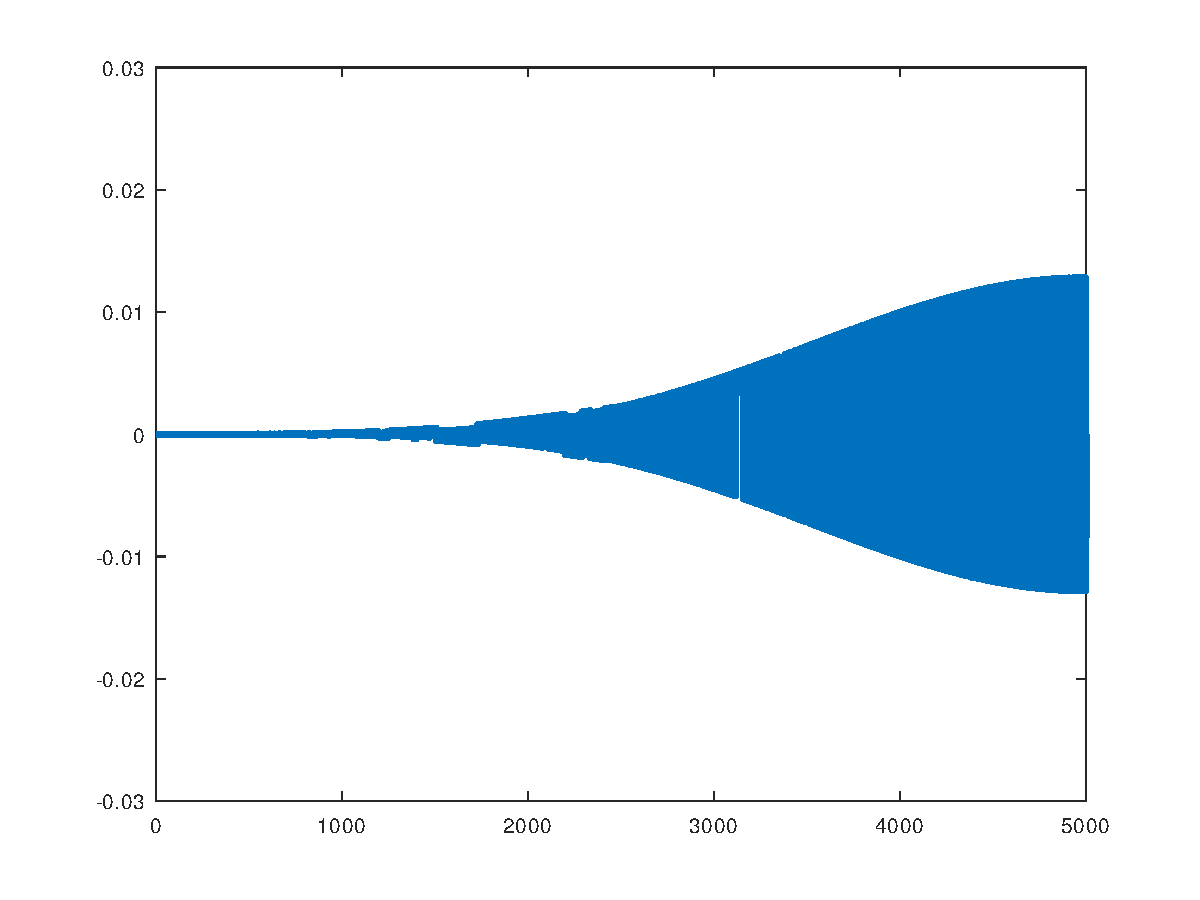
\includegraphics[
        width=\textwidth
        ]{papers/sgwt/images/dirac/dirac_gt1_gft.pdf}
        \vspace{-0pt}
        \caption{Eine mit $g(t\lambda)$, $t = 0.2$, modifizierte Fourier Graph 
        Transformierte eines Dirac-Stosses.
        \label{fig:sgwt:gft:gt1gft}}
    \end{minipage}
    ~
    \begin{minipage}[t]{0.49\textwidth}
        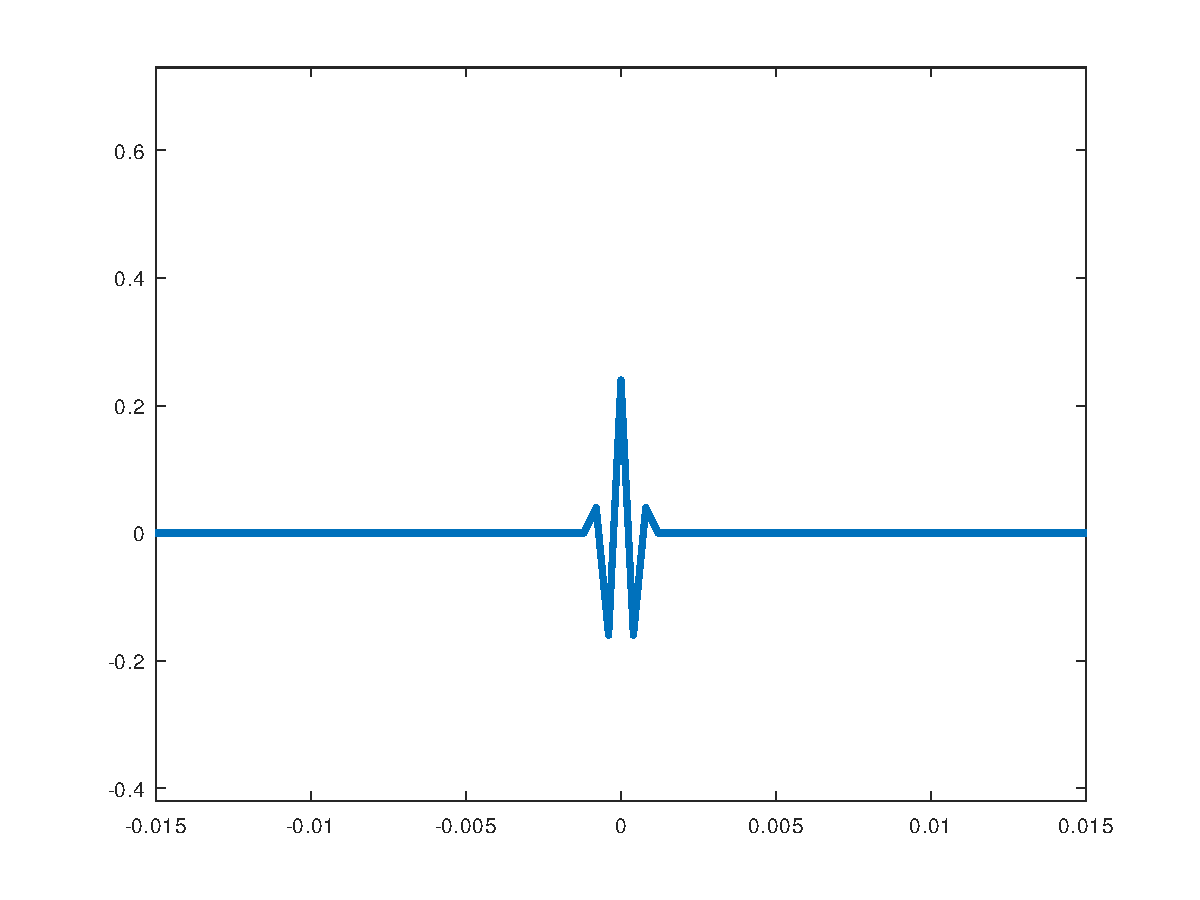
\includegraphics[
        width=\textwidth
        ]{papers/sgwt/images/dirac/dirac_gt1_igft.pdf}
        \vspace{-0pt}
        \caption{Das aus~\cref{fig:sgwt:gft:gt1gft} resultierende Wavelet.
        \label{fig:sgwt:gft:igt1gft}}
    \end{minipage}
    ~
    \begin{minipage}[t]{0.49\textwidth}
        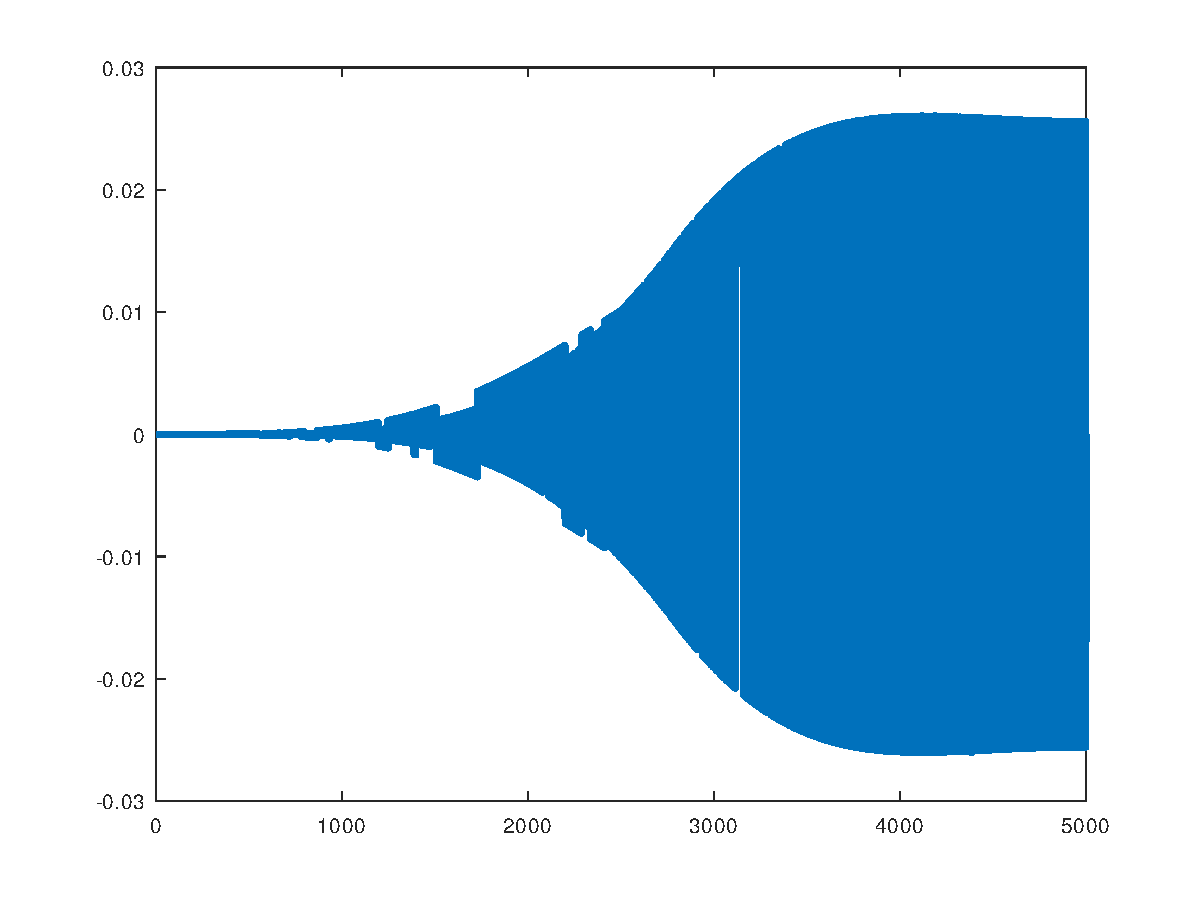
\includegraphics[
        width=\textwidth
        ]{papers/sgwt/images/dirac/dirac_gt2_gft.pdf}
        \vspace{-0pt}
        \caption{Eine mit $g(t\lambda)$, $t = 0.42295$, modifizierte Fourier 
        Graph-Transformierte eines Dirac-Stosses.
        \label{fig:sgwt:gft:gt2gft}}
    \end{minipage}
    ~
    \begin{minipage}[t]{0.49\textwidth}
        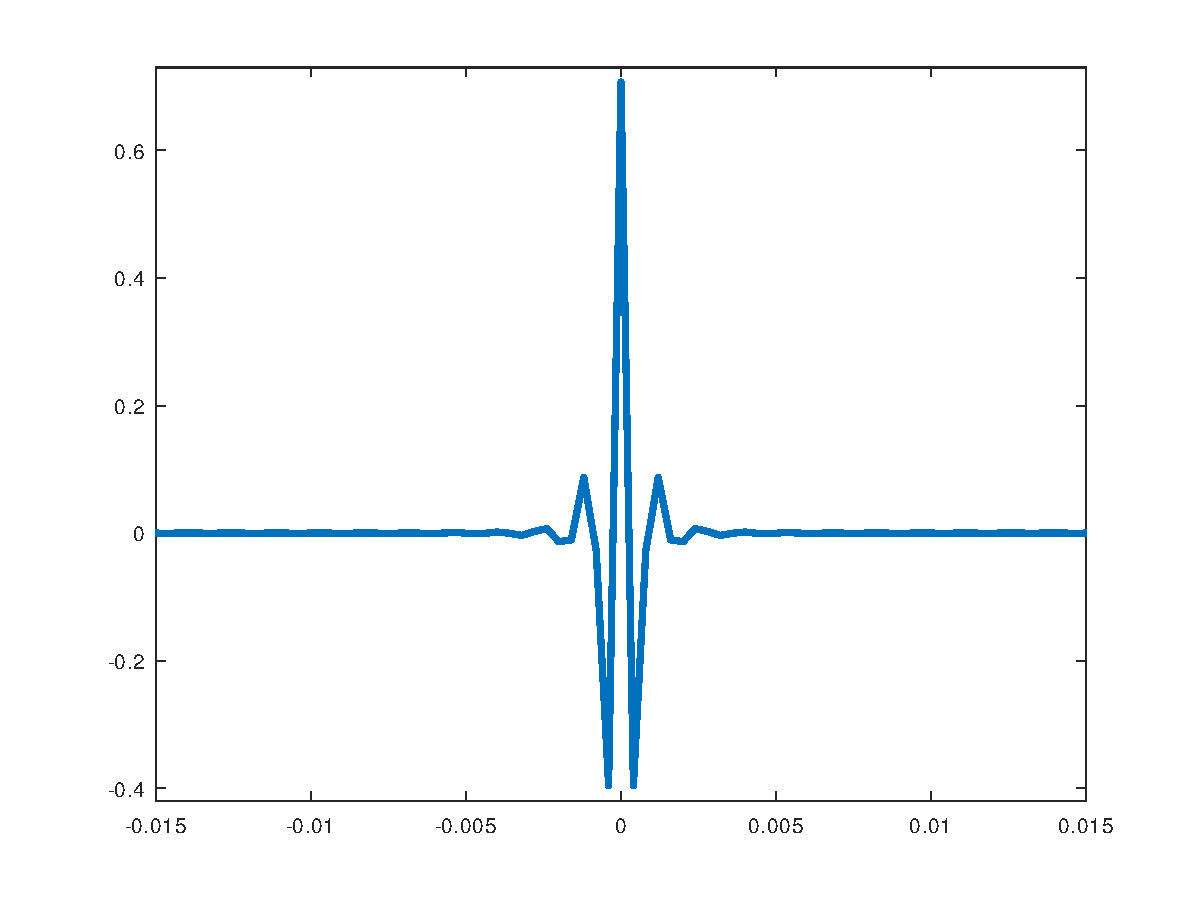
\includegraphics[
        width=\textwidth
        ]{papers/sgwt/images/dirac/dirac_gt2_igft.pdf}
        \vspace{-0pt}
        \caption{Das aus~\cref{fig:sgwt:gft:gt2gft} resultierende Wavelet.
        \label{fig:sgwt:gft:igt2gft}}
    \end{minipage}
    ~
    \begin{minipage}[t]{0.49\textwidth}
        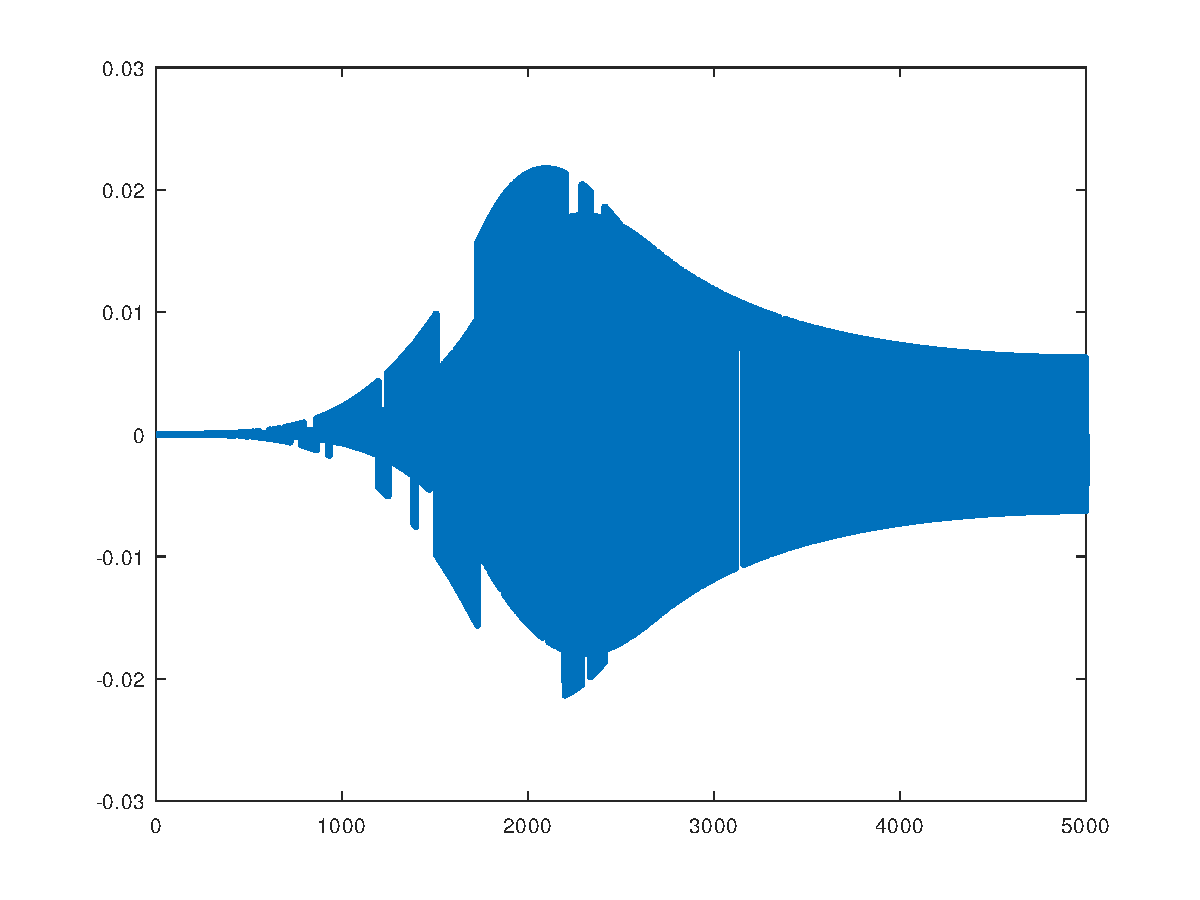
\includegraphics[
        width=\textwidth
        ]{papers/sgwt/images/dirac/dirac_gt3_gft.pdf}
        \vspace{-0pt}
        \caption{Eine mit $g(t\lambda)$, $t = 0.89443$, modifizierte Fourier 
        Graph-Transformierte eines Dirac-Stosses.
        \label{fig:sgwt:gft:gt3gft}}
    \end{minipage}
    ~
    \begin{minipage}[t]{0.49\textwidth}
        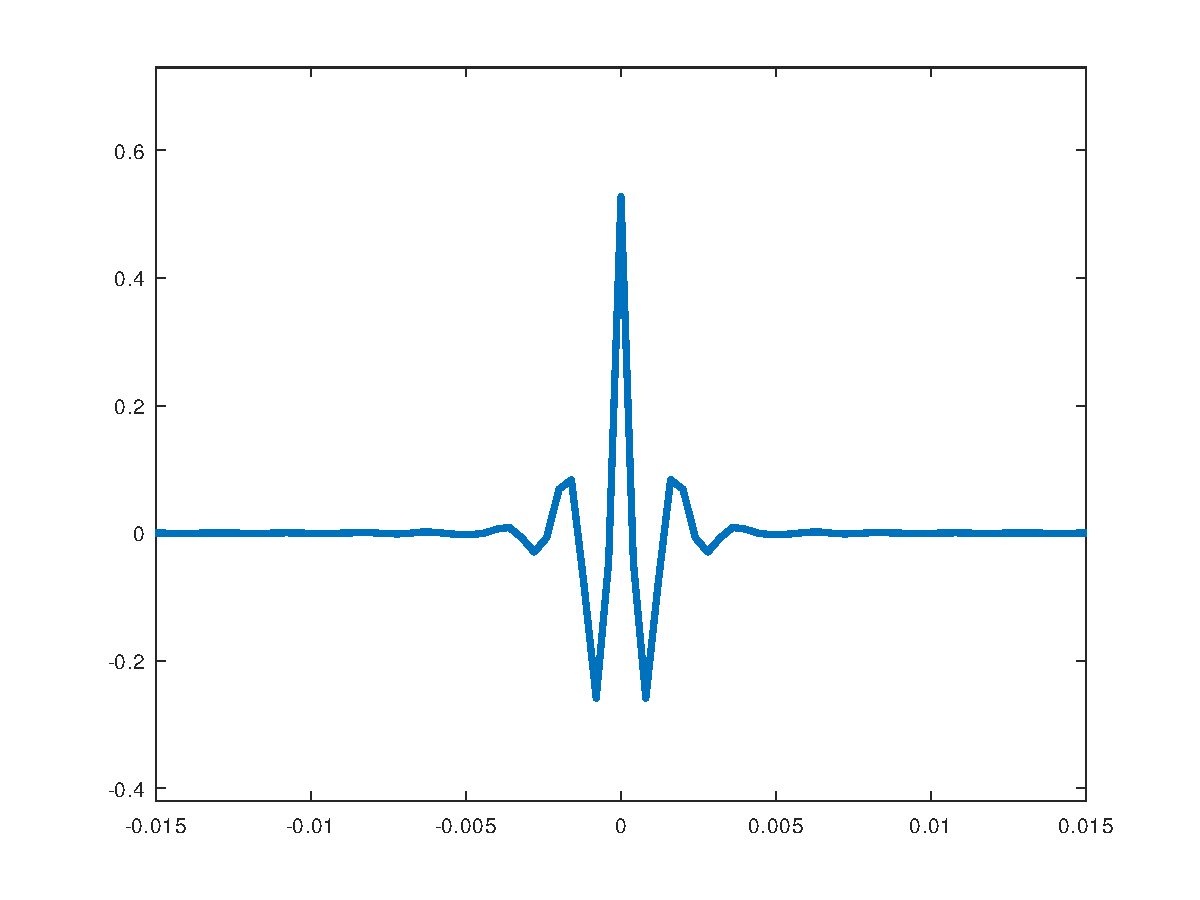
\includegraphics[
        width=\textwidth
        ]{papers/sgwt/images/dirac/dirac_gt3_igft.pdf}
        \vspace{-0pt}
        \caption{Das aus~\cref{fig:sgwt:gft:gt3gft} resultierende Wavelet.
        \label{fig:sgwt:gft:igt3gft}}
    \end{minipage}
\end{figure}
\begin{figure}
    \centering
    \begin{minipage}[t]{0.49\textwidth}
        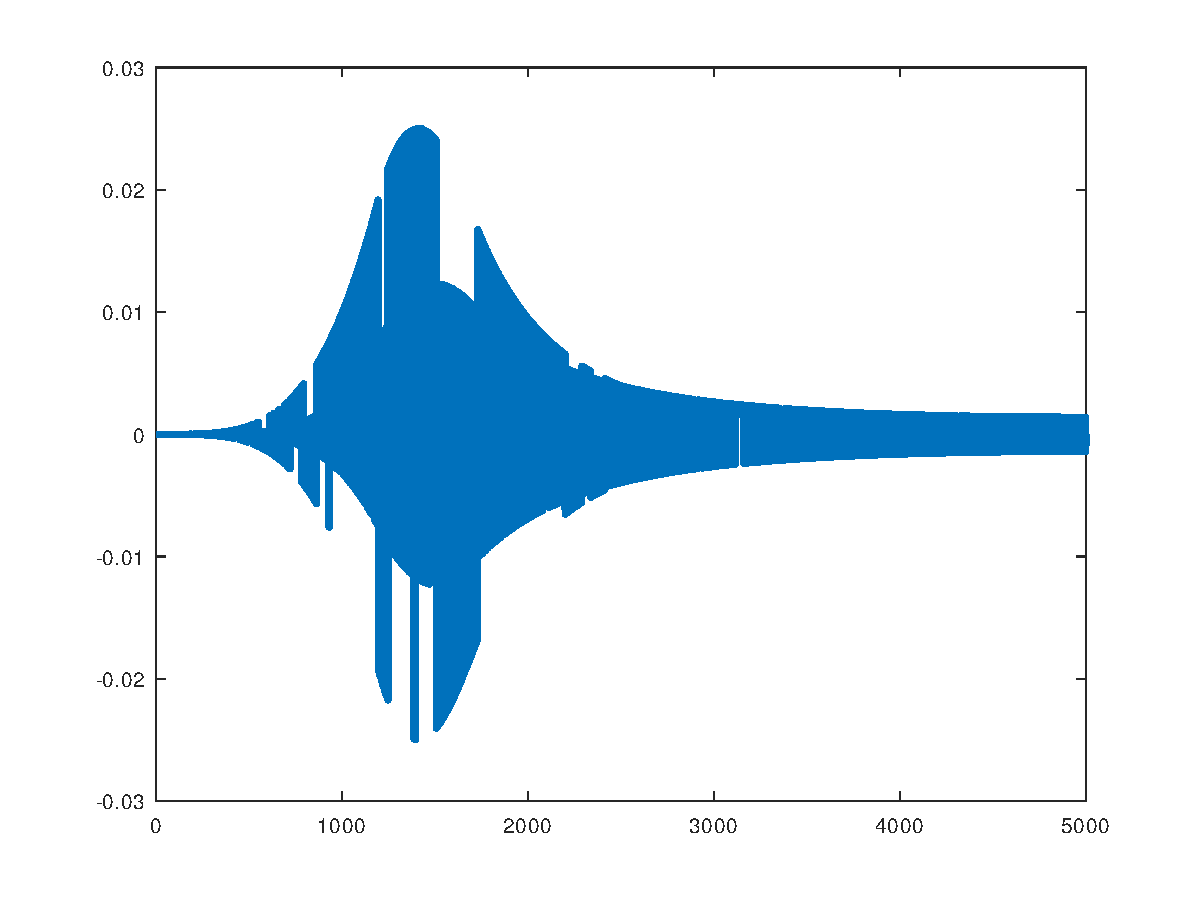
\includegraphics[
        width=\textwidth
        ]{papers/sgwt/images/dirac/dirac_gt4_gft.pdf}
        \vspace{-0pt}
        \caption{Eine mit $g(t\lambda)$, $t = 1.89148$, modifizierte Fourier 
        Graph-Transformierte eines Dirac-Stosses.
        \label{fig:sgwt:gft:gt4gft}}
    \end{minipage}
    ~
    \begin{minipage}[t]{0.49\textwidth}
        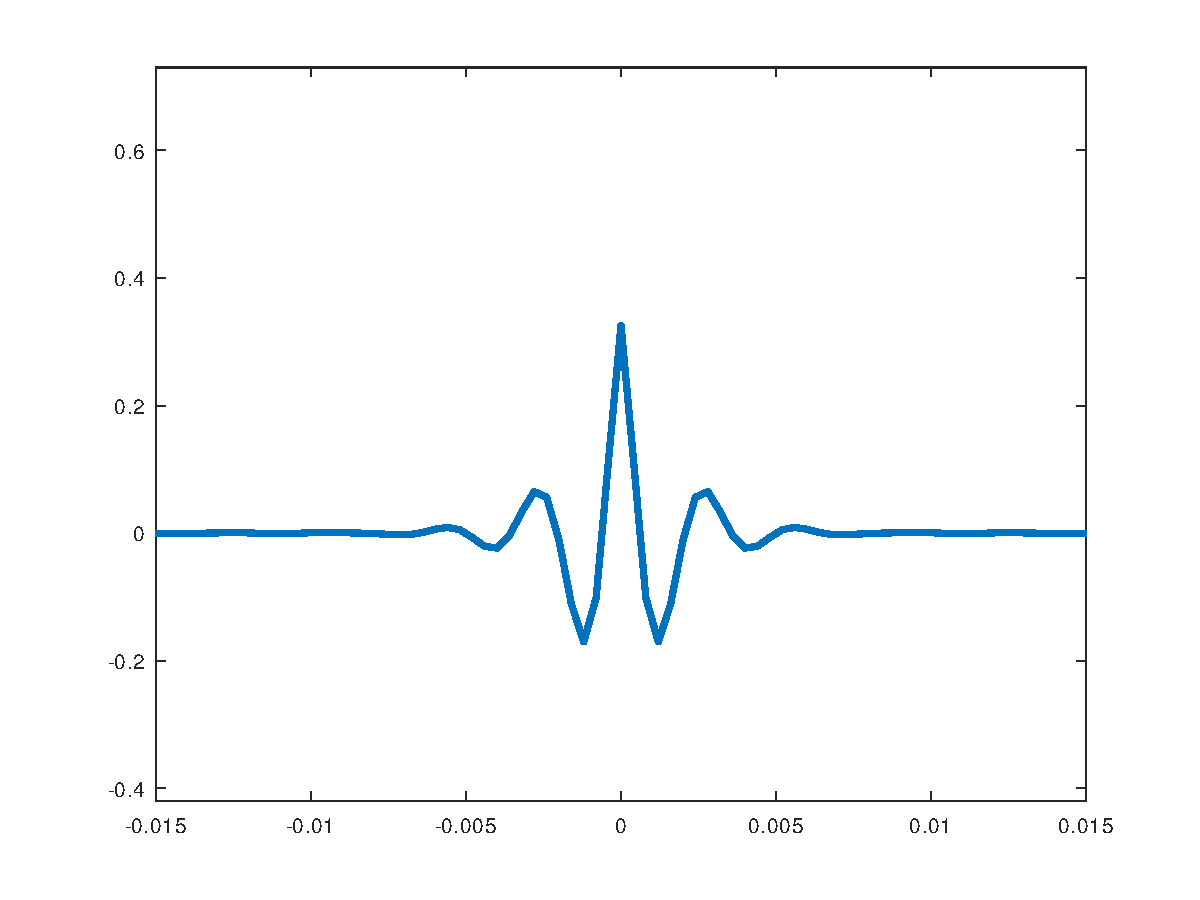
\includegraphics[
        width=\textwidth
        ]{papers/sgwt/images/dirac/dirac_gt4_igft.pdf}
        \vspace{-0pt}
        \caption{Das aus~\cref{fig:sgwt:gft:gt4gft} resultierende Wavelet.
        \label{fig:sgwt:gft:igt4gft}}
    \end{minipage}
    ~
    \begin{minipage}[t]{0.49\textwidth}
        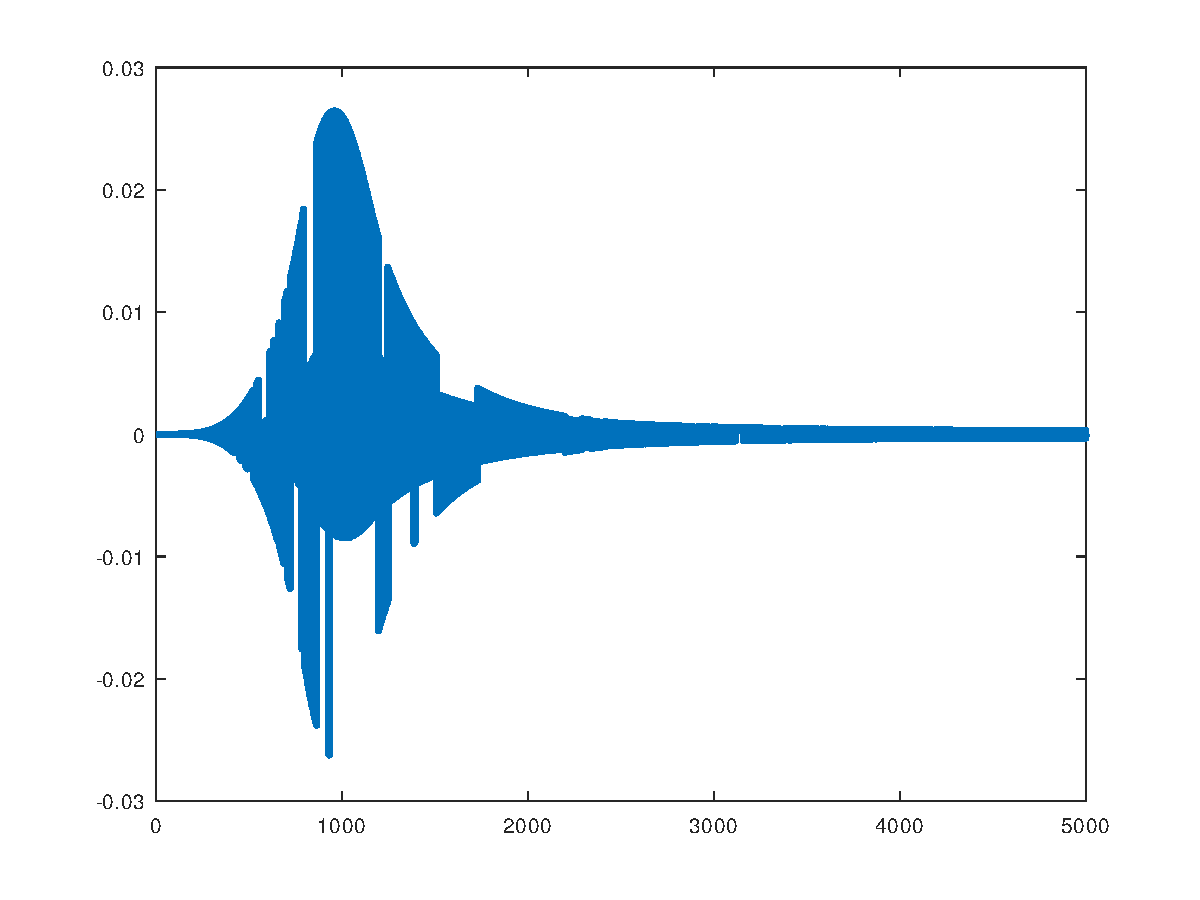
\includegraphics[
        width=\textwidth
        ]{papers/sgwt/images/dirac/dirac_gt5_gft.pdf}
        \vspace{-0pt}
        \caption{Eine mit $g(t\lambda)$, $t = 4$, modifizierte Fourier Graph 
        Transformierte eines Dirac-Stosses.
        \label{fig:sgwt:gft:gt5gft}}
    \end{minipage}
    ~
    \begin{minipage}[t]{0.49\textwidth}
        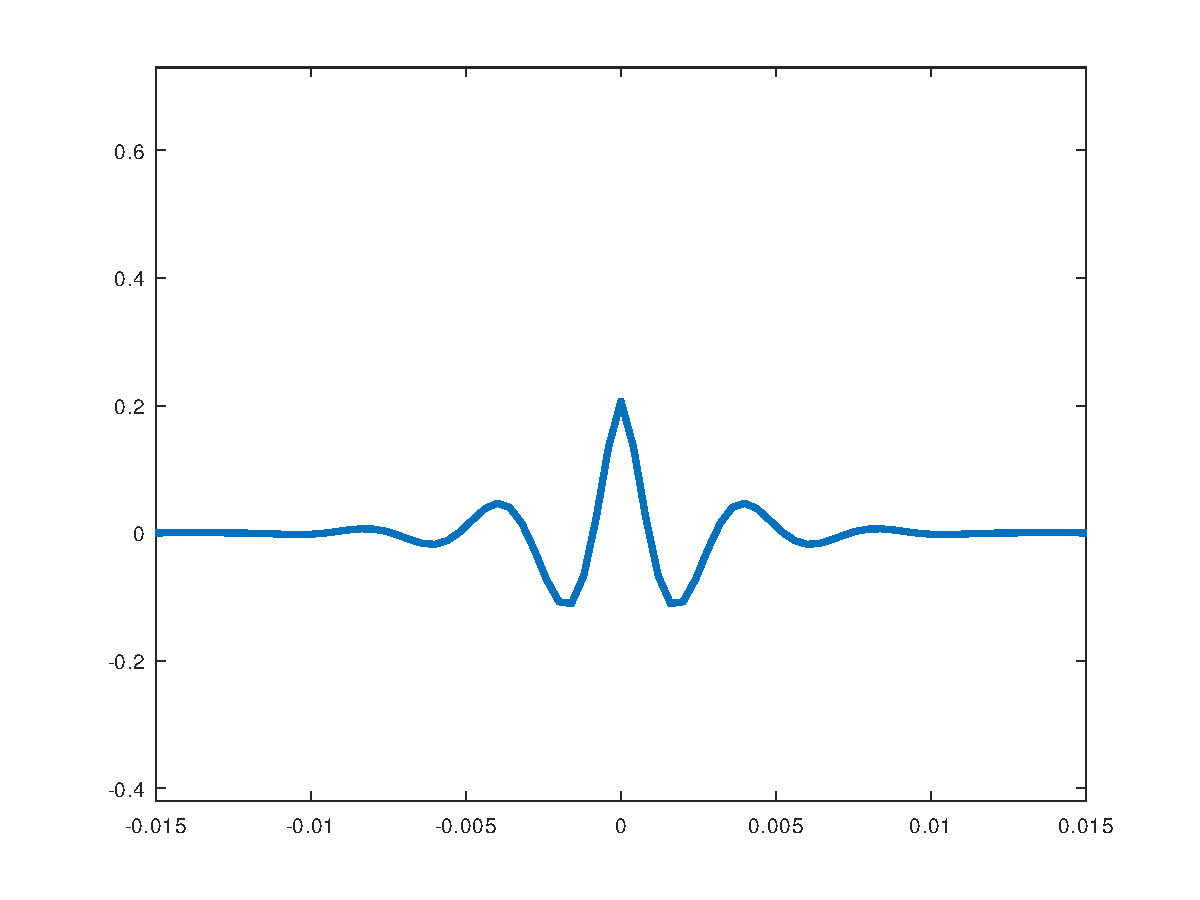
\includegraphics[
        width=\textwidth
        ]{papers/sgwt/images/dirac/dirac_gt5_igft.pdf}
        \vspace{-0pt}
        \caption{Das aus~\cref{fig:sgwt:gft:gt5gft} resultierende Wavelet.
        \label{fig:sgwt:gft:igt5gft}}
    \end{minipage}
\end{figure}

Die $t$ entsprechen somit genau dem $a$ in der klassischen 
Wavelet-Transformation. Es dr\"uckt die ``Verbreiterung'' des Wavelets aus.
Die Translation $b$ der klassischen Transformation kann man dagegen nicht 
retten, denn die Existenz des $b$ in der klassischen Transformation drückt ja 
aus, dass man die Analyse an jedem Punkt des Definitionsbereichs mit der 
``gleichen'' Funktion machen kann. Das ist aber auf einem Graphen 
grunds\"atzlich nicht m\"oglich, denn man kann die Eigenfunktionen nicht 
miteinander vergleichen.

\begin{figure}
    \centering
    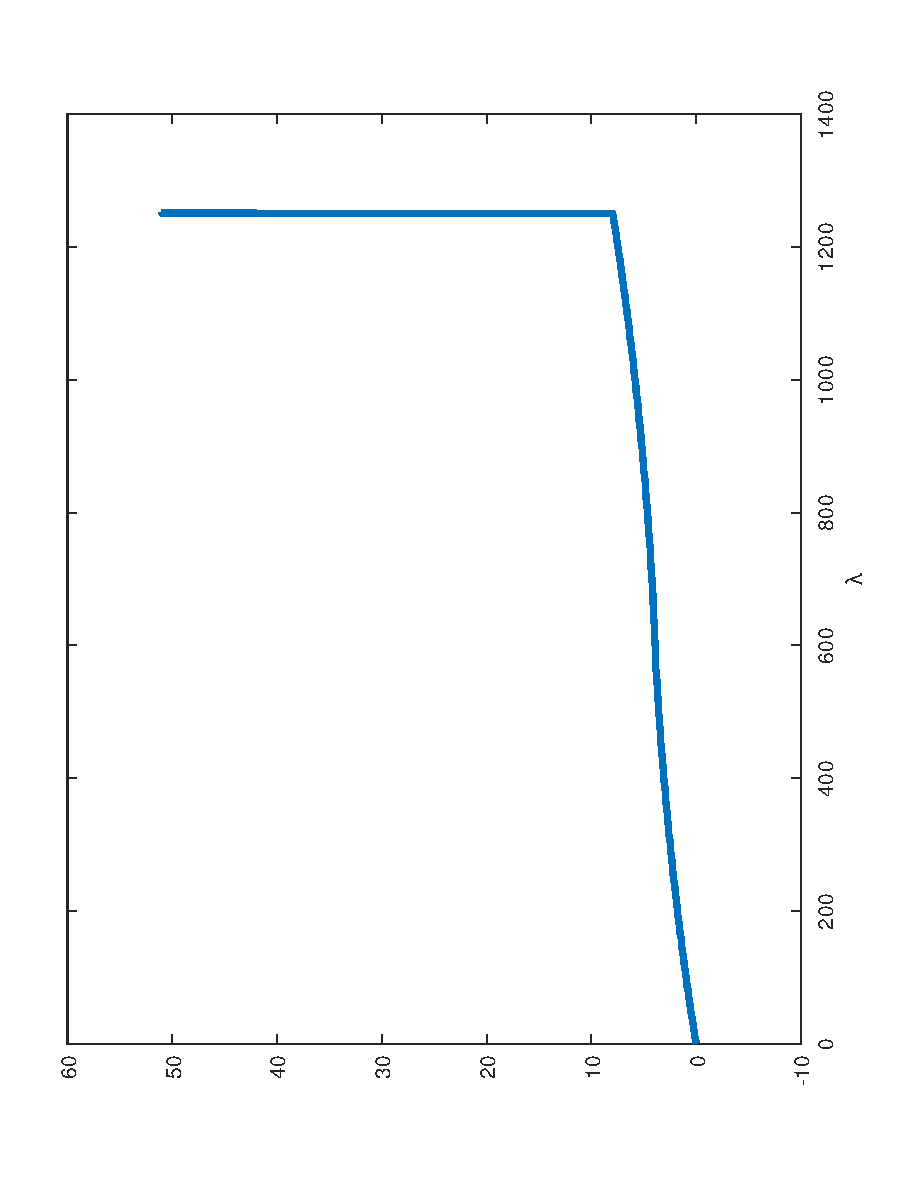
\includegraphics[
    angle=-90,
    origin=c,
    scale=0.6
    ]{papers/sgwt/images/wavelets/lambda.pdf}
    \vspace{-50pt}
    \caption{Eigenwerte $\lambda$ eines Kugelgraphen mit 1252 Knoten. 
        \label{fig:sgwt:wavelets:sphere:lambda}}
\end{figure}

\begin{figure}
    \begin{minipage}[t]{0.49\textwidth}
        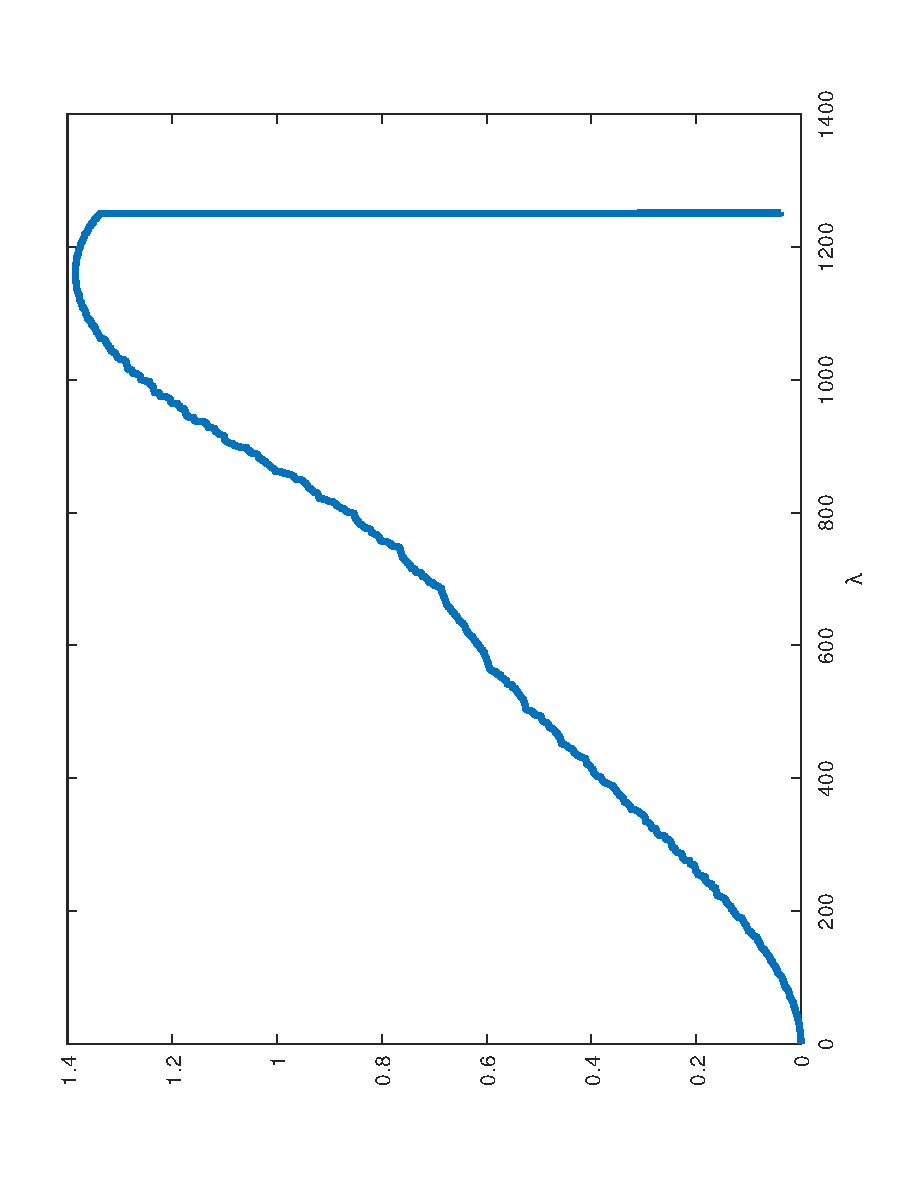
\includegraphics[
        angle=-90,
        origin=c,
        width=\textwidth]{papers/sgwt/images/wavelets/gt1.pdf}
        \vspace{-45pt}
        \caption{Die Kernelfunktion $g(t_1\lambda)$ eines Kugelgraphen mit 1252 
            Knoten und $t_1 = 0.2$.}
        \label{fig:sgwt:wavelets:sphere:gt1}
    \end{minipage}
    ~
    \begin{minipage}[t]{0.49\textwidth}
        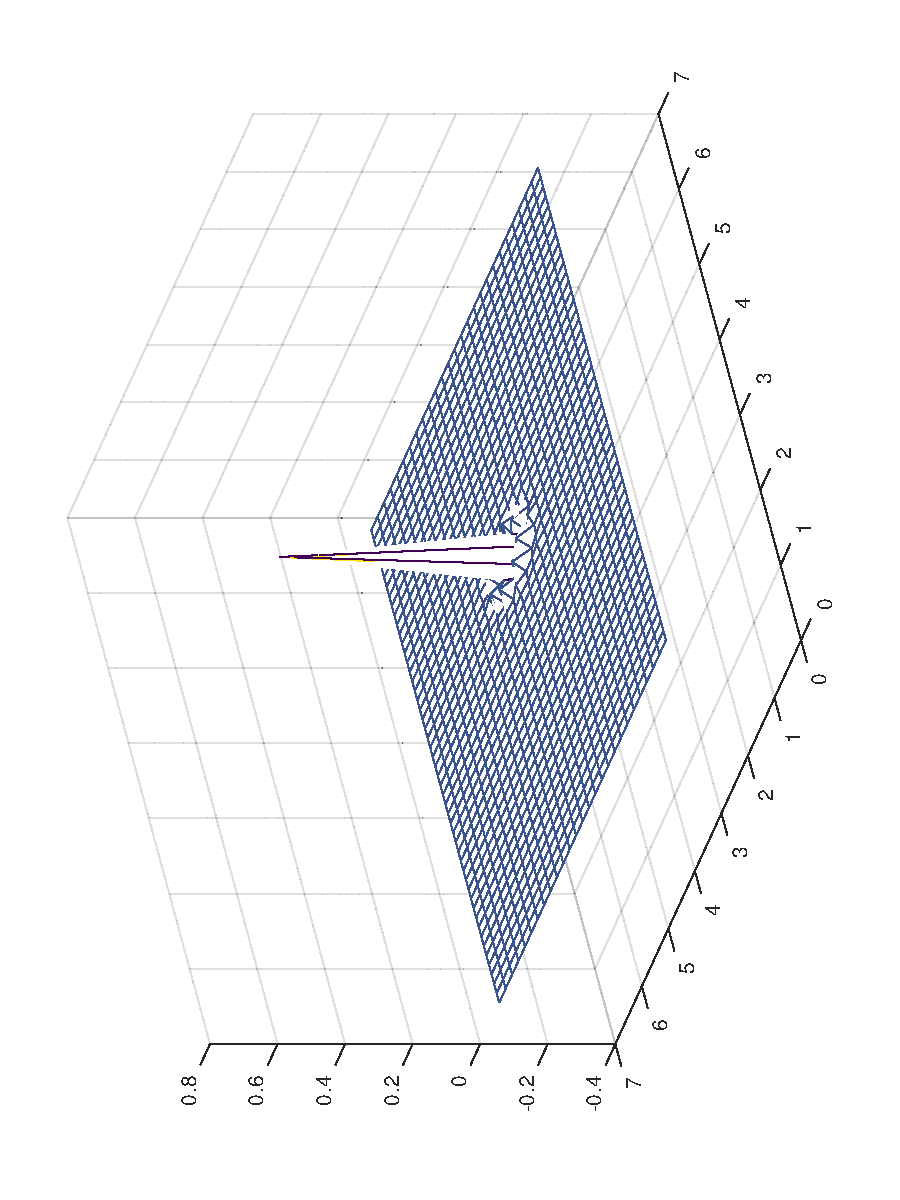
\includegraphics[
        angle=-90,
        origin=c,
        width=\textwidth]{papers/sgwt/images/wavelets/psi_t1_50_25_630_flat.pdf}
        \vspace{-45pt}
        \caption{$\psi_1(v_{630})$-Wavelet eines Kugelgraphen mit 1252 Knoten.}
        \label{fig:sgwt:wavelets:sphere:psi1:flat}
    \end{minipage}
    ~
    \begin{minipage}[t]{\textwidth}
        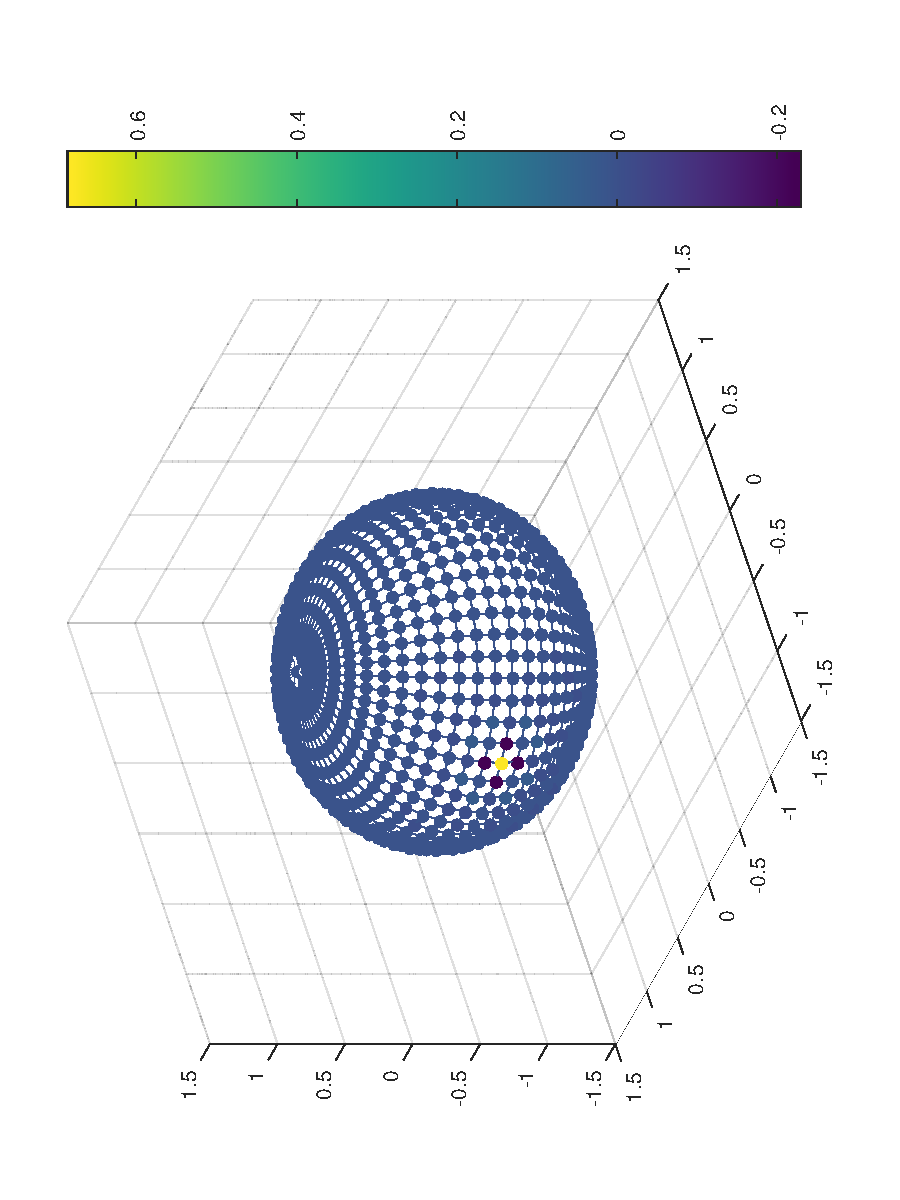
\includegraphics[
        angle=-90,
        origin=c,
        width=\textwidth]{papers/sgwt/images/wavelets/psi_t1_50_25_630.pdf}
        \vspace{-45pt}
        \caption{$\psi_1(v_{630})$-Wavelet eines Kugelgraphen mit 1252 Knoten.}
        \label{fig:sgwt:wavelets:sphere:psi1}
    \end{minipage}
\end{figure}

\begin{figure}
    \begin{minipage}[t]{0.49\textwidth}
        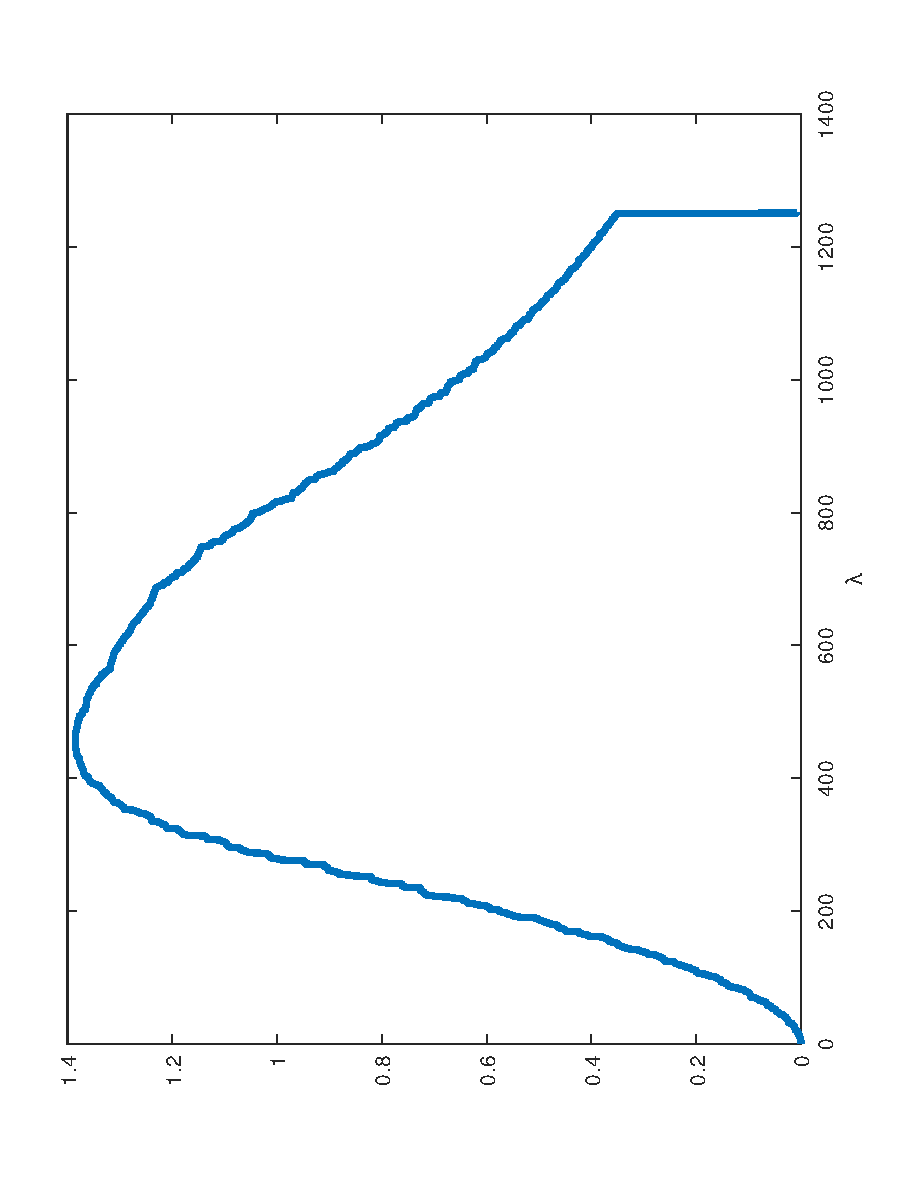
\includegraphics[
        angle=-90,
        origin=c,
        width=\textwidth]{papers/sgwt/images/wavelets/gt2.pdf}
        \vspace{-45pt}
        \caption{Die Kernelfunktion $g(t_2\lambda)$ eines Kugelgraphen mit 1252 
            Knoten und $t_2 = 0.42295$.}
        \label{fig:sgwt:wavelets:sphere:gt2}
    \end{minipage}
    ~
    \begin{minipage}[t]{0.49\textwidth}
        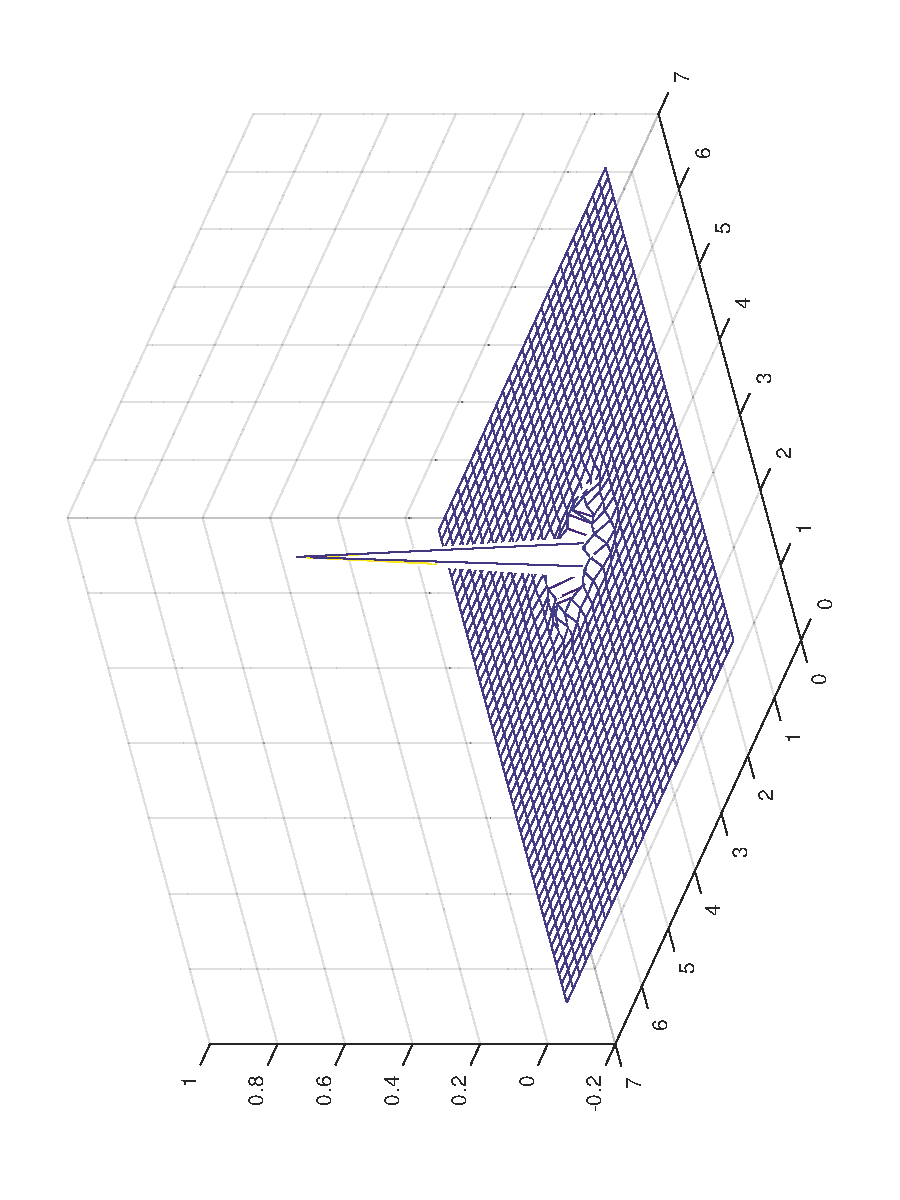
\includegraphics[
        angle=-90,
        origin=c,
        width=\textwidth]{papers/sgwt/images/wavelets/psi_t2_50_25_630_flat.pdf}
        \vspace{-45pt}
        \caption{$\psi_2(v_{630})$-Wavelet eines Kugelgraphen mit 1252 Knoten.}
        \label{fig:sgwt:wavelets:sphere:psi2:flat}
    \end{minipage}
    ~
    \begin{minipage}[t]{\textwidth}
        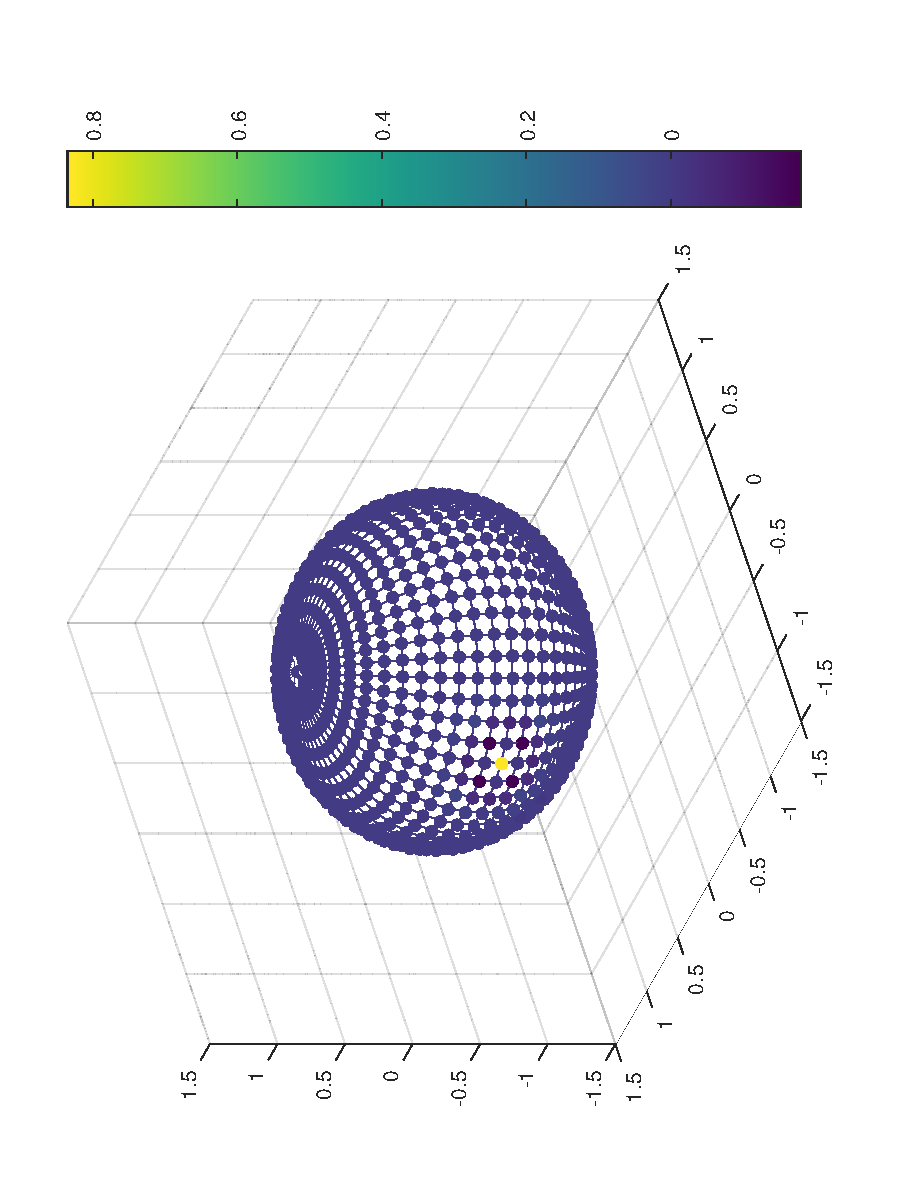
\includegraphics[
        angle=-90,
        origin=c,
        width=\textwidth]{papers/sgwt/images/wavelets/psi_t2_50_25_630.pdf}
        \vspace{-45pt}
        \caption{$\psi_2(v_{630})$-Wavelet eines Kugelgraphen mit 1252 Knoten.}
        \label{fig:sgwt:wavelets:sphere:psi2}
    \end{minipage}
\end{figure}

\begin{figure}
    \begin{minipage}[t]{0.49\textwidth}
        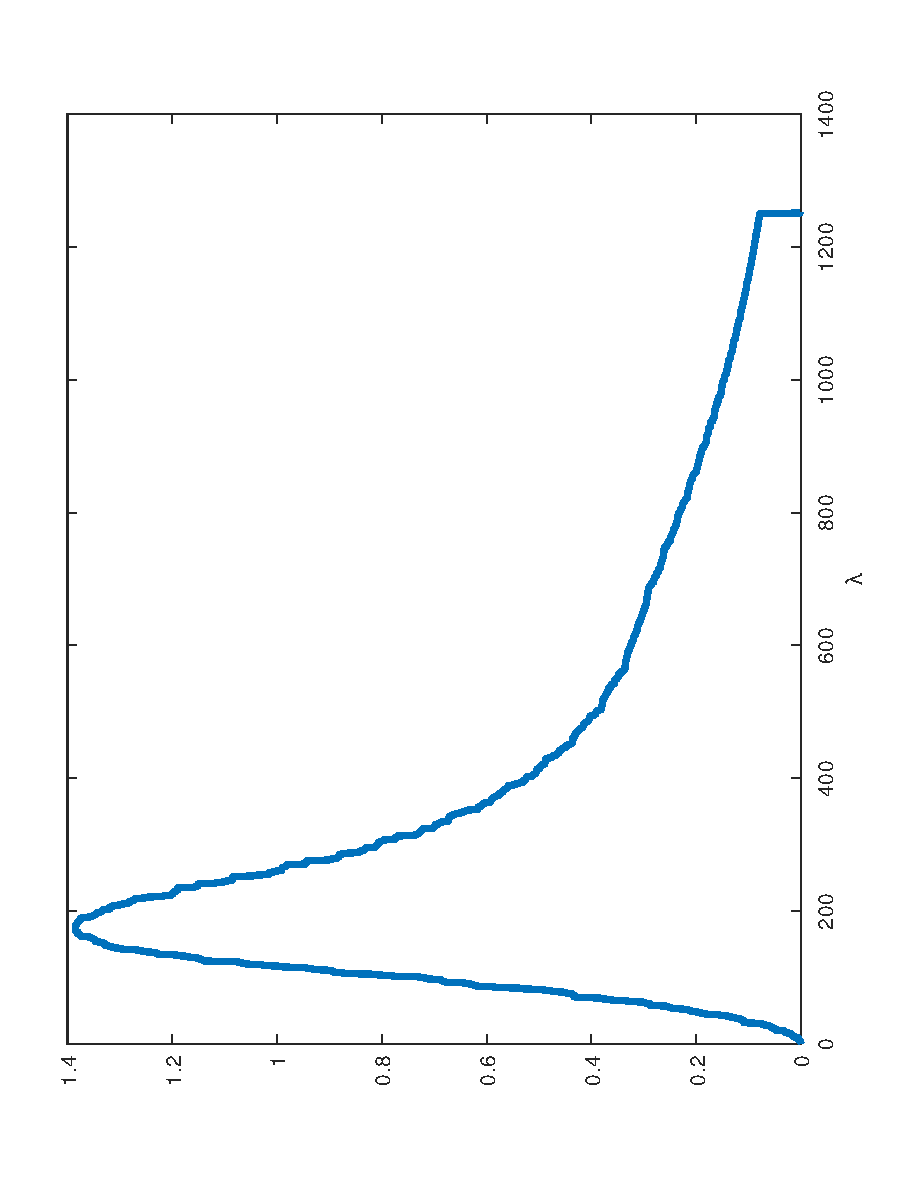
\includegraphics[
        angle=-90,
        origin=c,
        width=\textwidth]{papers/sgwt/images/wavelets/gt3.pdf}
        \vspace{-45pt}
        \caption{Die Kernelfunktion $g(t_3\lambda)$ eines Kugelgraphen mit 1252 
            Knoten und $t_3 = 0.89443$.}
        \label{fig:sgwt:wavelets:sphere:gt3}
    \end{minipage}
    ~
    \begin{minipage}[t]{0.49\textwidth}
        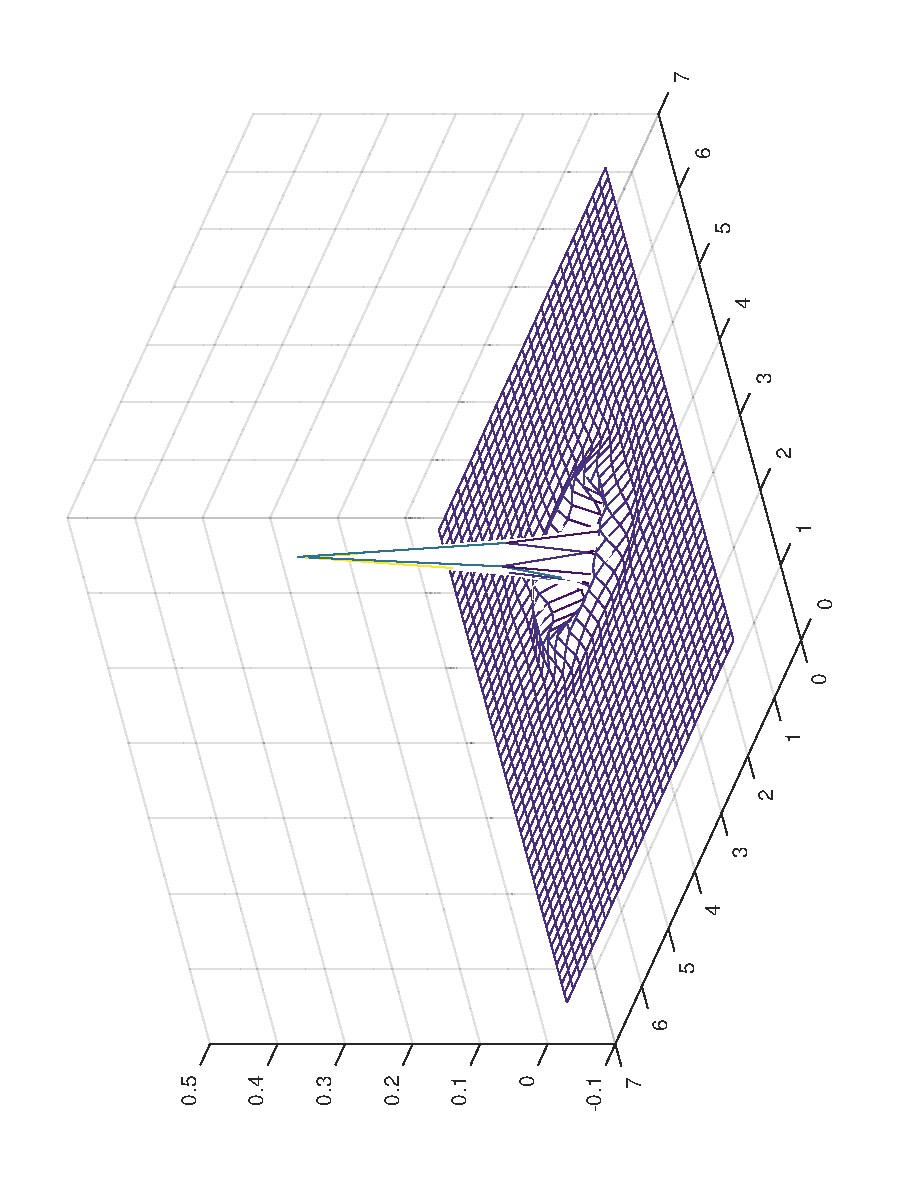
\includegraphics[
        angle=-90,
        origin=c,
        width=\textwidth]{papers/sgwt/images/wavelets/psi_t3_50_25_630_flat.pdf}
        \vspace{-45pt}
        \caption{$\psi_3(v_{630})$-Wavelet eines Kugelgraphen mit 1252 Knoten.}
        \label{fig:sgwt:wavelets:sphere:psi3:flat}
    \end{minipage}
    ~
    \begin{minipage}[t]{\textwidth}
        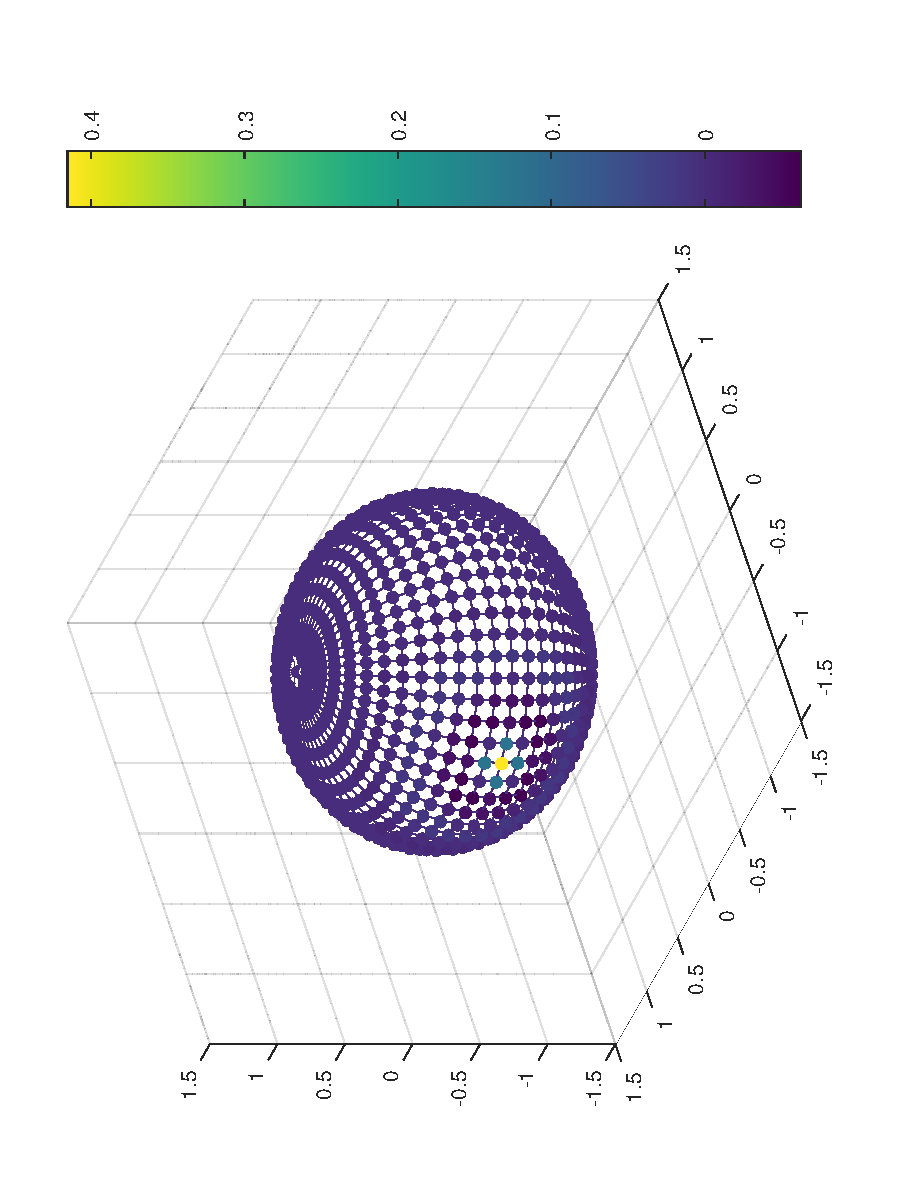
\includegraphics[
        angle=-90,
        origin=c,
        width=\textwidth]{papers/sgwt/images/wavelets/psi_t3_50_25_630.pdf}
        \vspace{-45pt}
        \caption{$\psi_3(v_{630})$-Wavelet eines Kugelgraphen mit 1252 Knoten.}
        \label{fig:sgwt:wavelets:sphere:psi3}
    \end{minipage}
\end{figure}

\begin{figure}
    \begin{minipage}[t]{0.49\textwidth}
        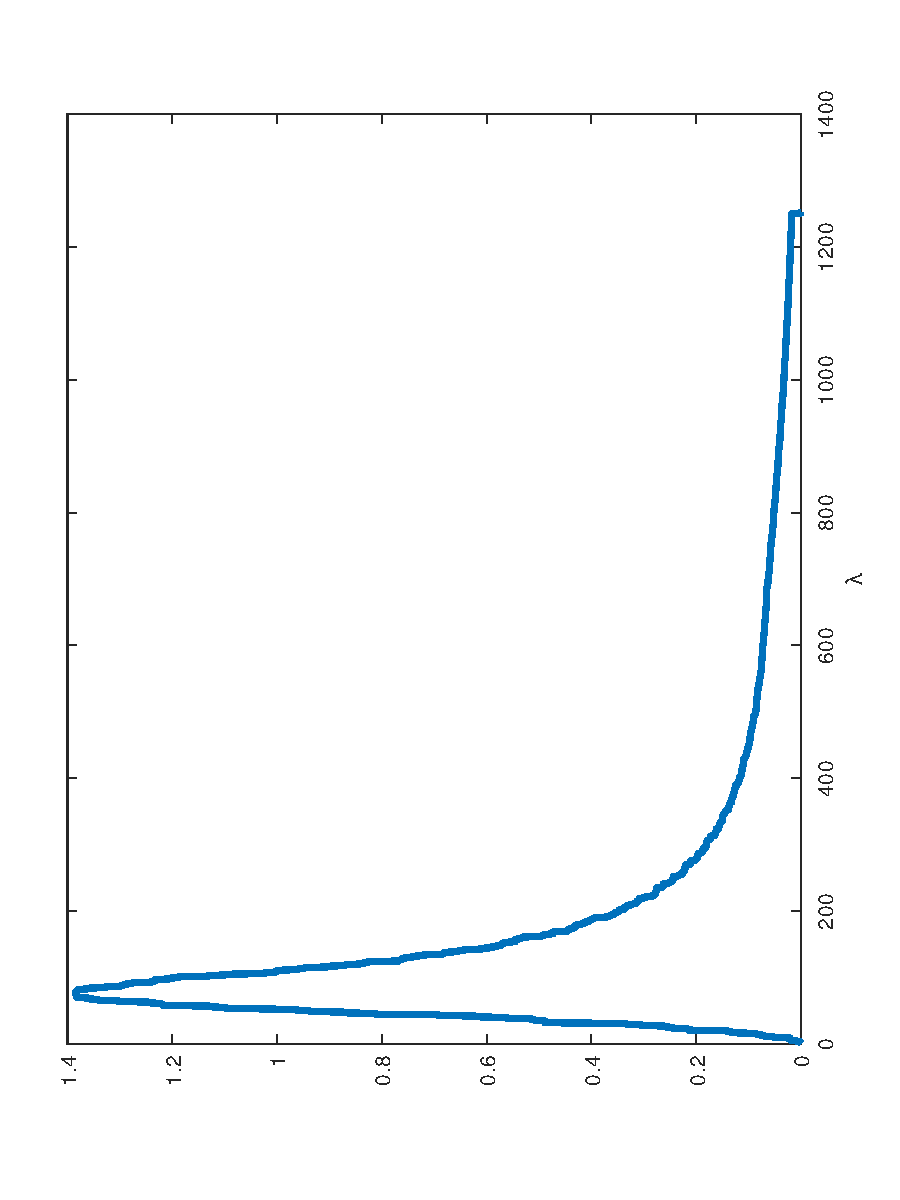
\includegraphics[
        angle=-90,
        origin=c,
        width=\textwidth]{papers/sgwt/images/wavelets/gt4.pdf}
        \vspace{-45pt}
        \caption{Die Kernelfunktion $g(t_4\lambda)$ eines Kugelgraphen mit 1252 
            Knoten und $t_4 = 1.89148$.}
        \label{fig:sgwt:wavelets:sphere:gt4}
    \end{minipage}
    ~
    \begin{minipage}[t]{0.49\textwidth}
        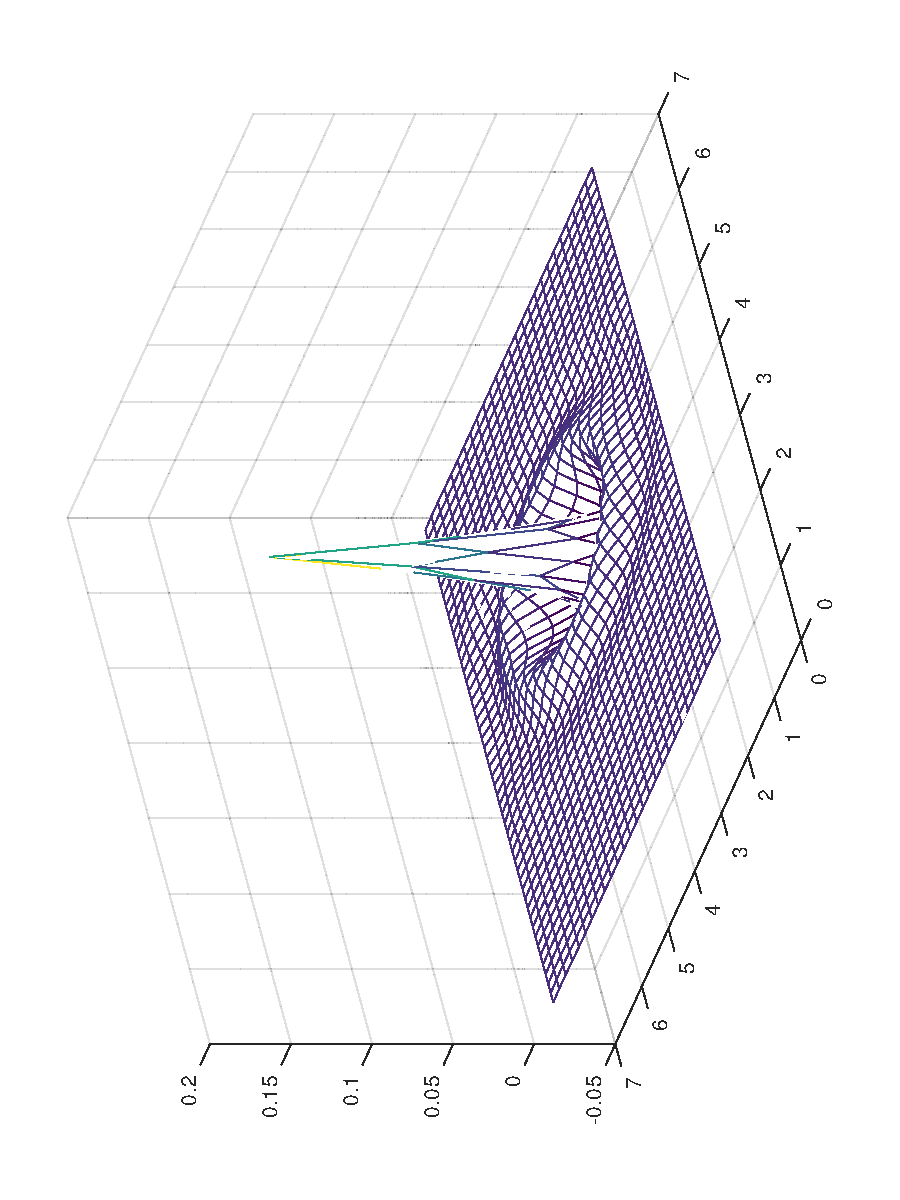
\includegraphics[
        angle=-90,
        origin=c,
        width=\textwidth]{papers/sgwt/images/wavelets/psi_t4_50_25_630_flat.pdf}
        \vspace{-45pt}
        \caption{$\psi_4(v_{630})$-Wavelet eines Kugelgraphen mit 1252 Knoten.}
        \label{fig:sgwt:wavelets:sphere:psi4:flat}
    \end{minipage}
    ~
    \begin{minipage}[t]{\textwidth}
        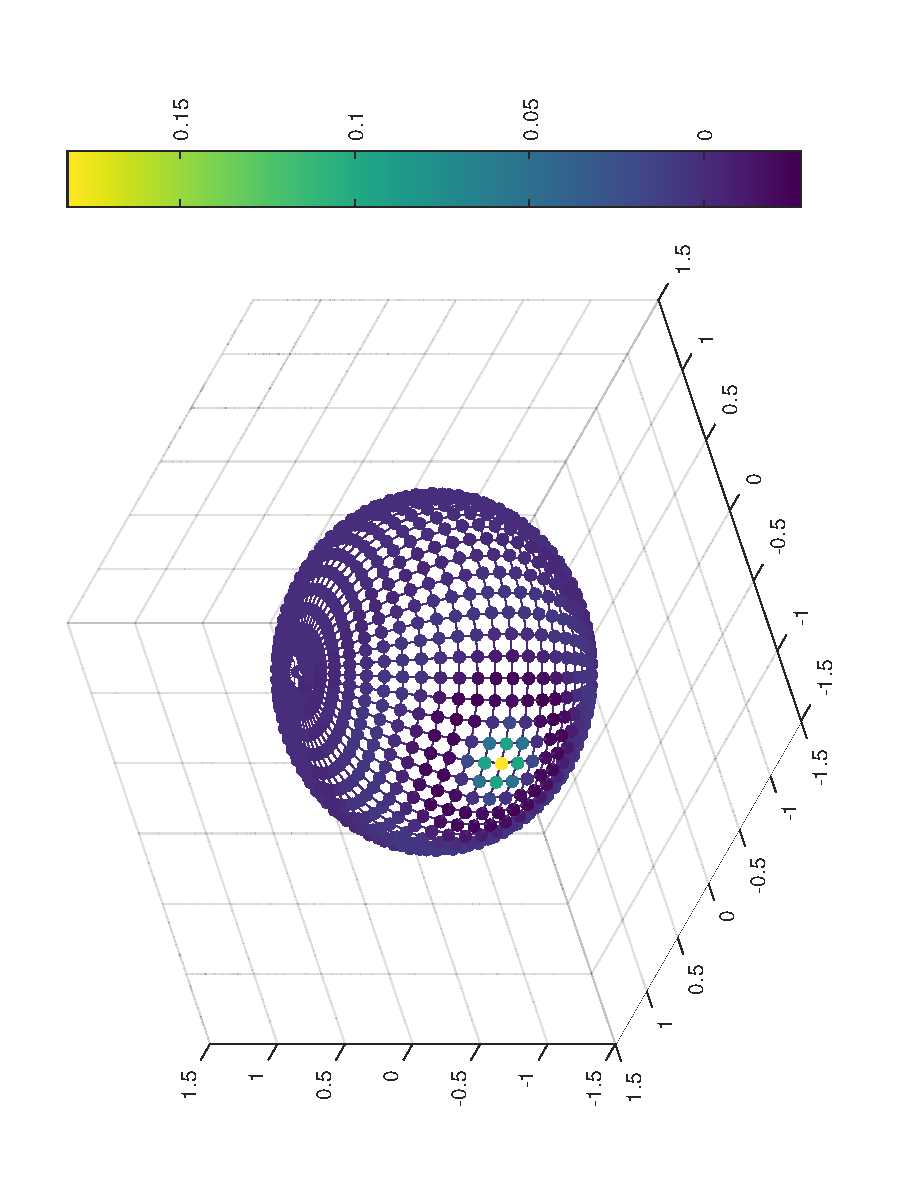
\includegraphics[
        angle=-90,
        origin=c,
        width=\textwidth]{papers/sgwt/images/wavelets/psi_t4_50_25_630.pdf}
        \vspace{-45pt}
        \caption{$\psi_4(v_{630})$-Wavelet eines Kugelgraphen mit 1252 Knoten.}
        \label{fig:sgwt:wavelets:sphere:psi4}
    \end{minipage}
\end{figure}

\begin{figure}
    \begin{minipage}[t]{0.49\textwidth}
        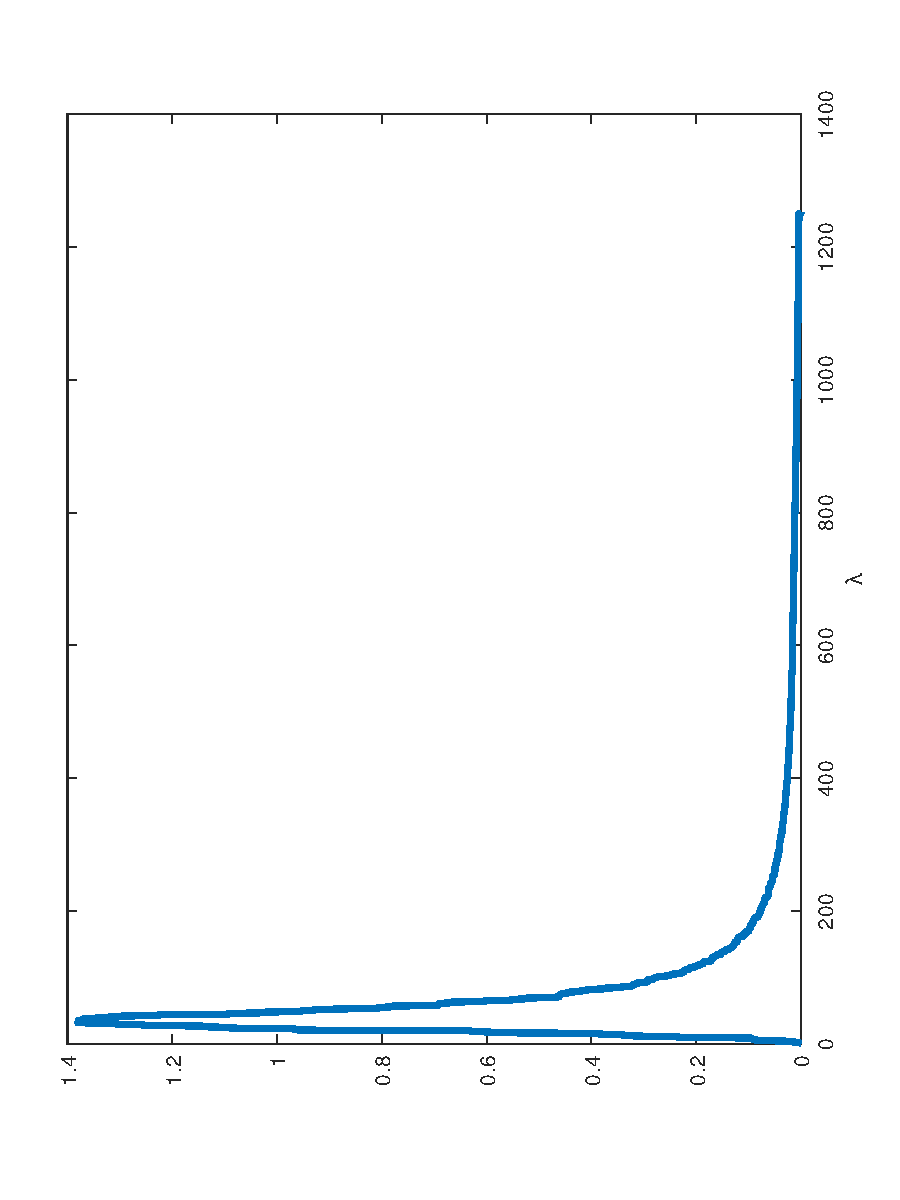
\includegraphics[
        angle=-90,
        origin=c,
        width=\textwidth]{papers/sgwt/images/wavelets/gt5.pdf}
        \vspace{-45pt}
        \caption{Die Kernelfunktion $g(t_5\lambda)$ eines Kugelgraphen mit 1252 
            Knoten und $t_5 = 4$.}
        \label{fig:sgwt:wavelets:sphere:gt5}
    \end{minipage}
    ~
    \begin{minipage}[t]{0.49\textwidth}
        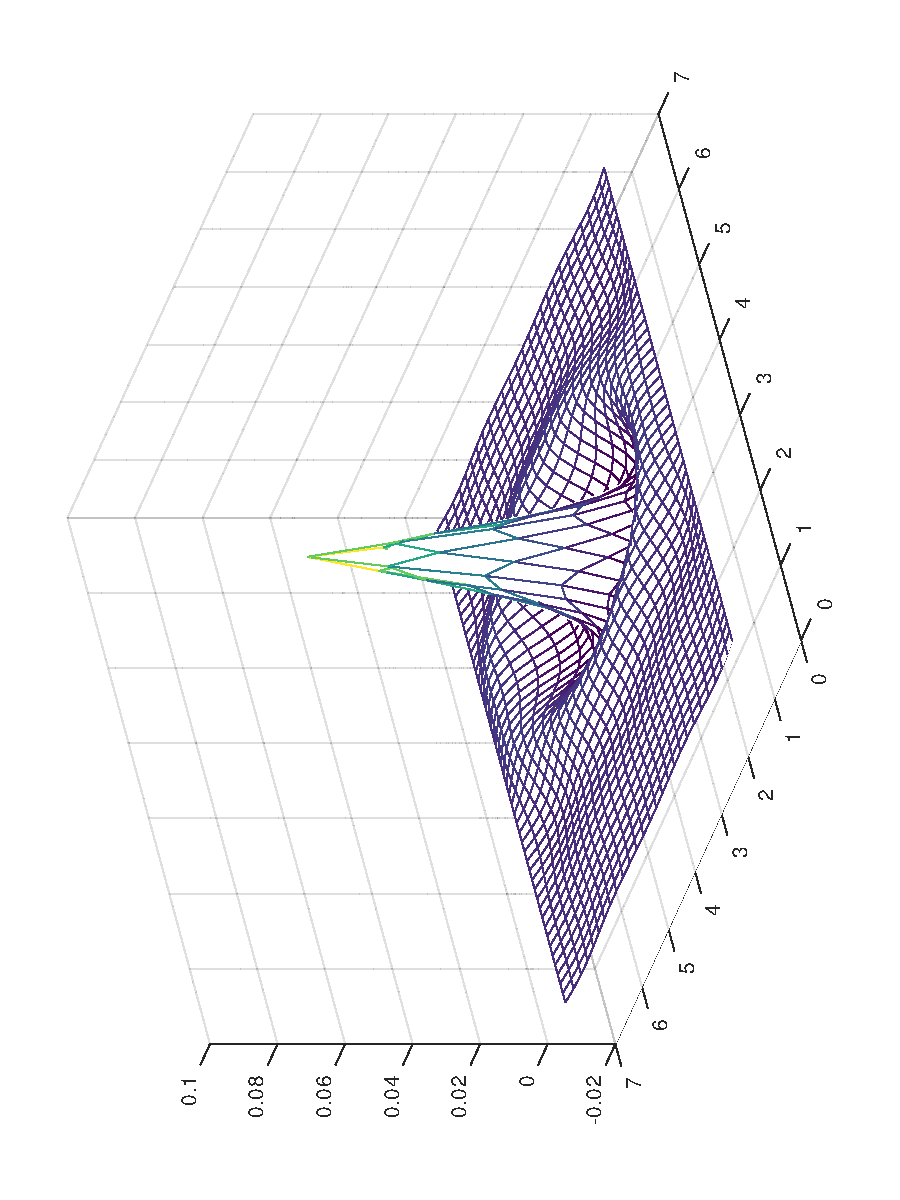
\includegraphics[
        angle=-90,
        origin=c,
        width=\textwidth]{papers/sgwt/images/wavelets/psi_t5_50_25_630_flat.pdf}
        \vspace{-45pt}
        \caption{$\psi_5(v_{630})$-Wavelet eines Kugelgraphen mit 1252 Knoten.}
        \label{fig:sgwt:wavelets:sphere:psi5:flat}
    \end{minipage}
    ~
    \begin{minipage}[t]{\textwidth}
        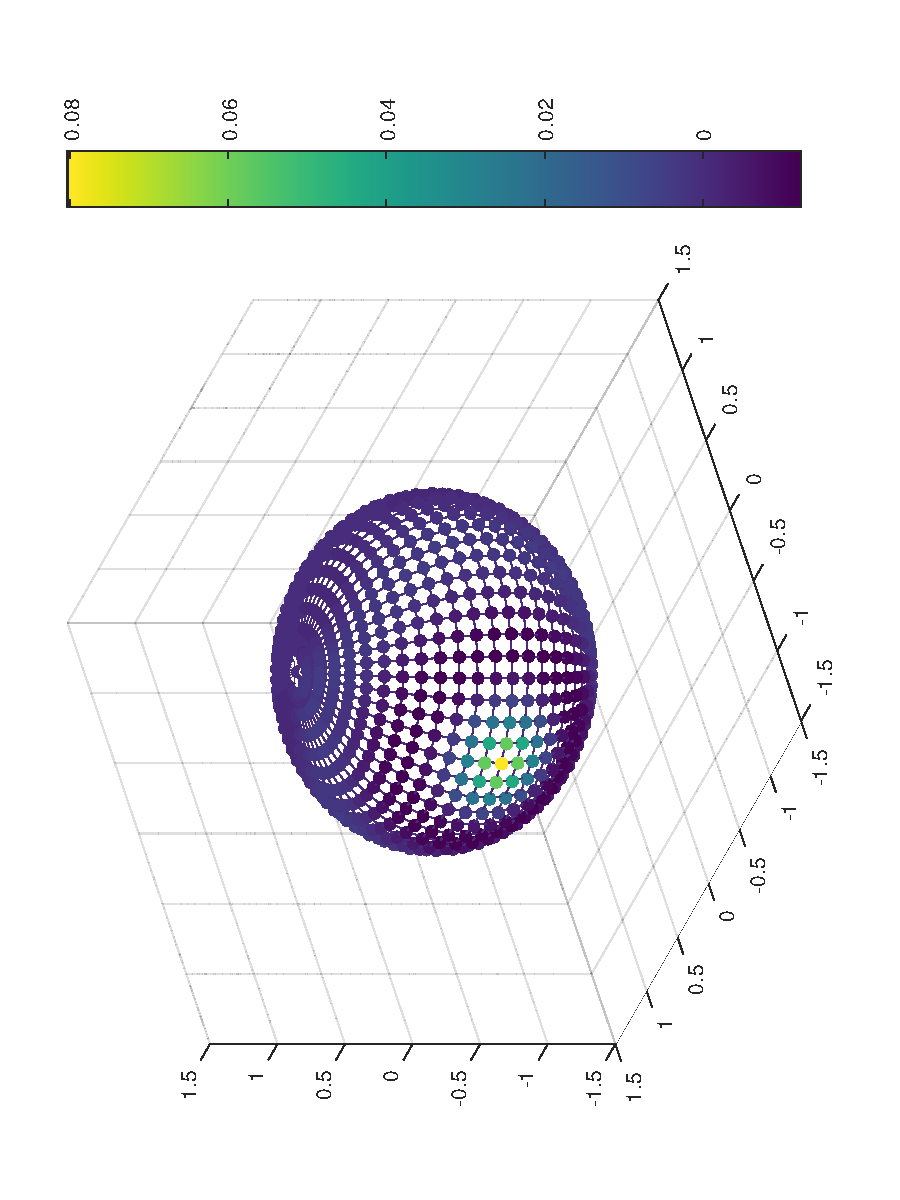
\includegraphics[
        angle=-90,
        origin=c,
        width=\textwidth]{papers/sgwt/images/wavelets/psi_t5_50_25_630.pdf}
        \vspace{-45pt}
        \caption{$\psi_5(v_{630})$-Wavelet eines Kugelgraphen mit 1252 Knoten.}
        \label{fig:sgwt:wavelets:sphere:psi5}
    \end{minipage}
\end{figure}

\begin{figure}
    \begin{minipage}[t]{0.49\textwidth}
        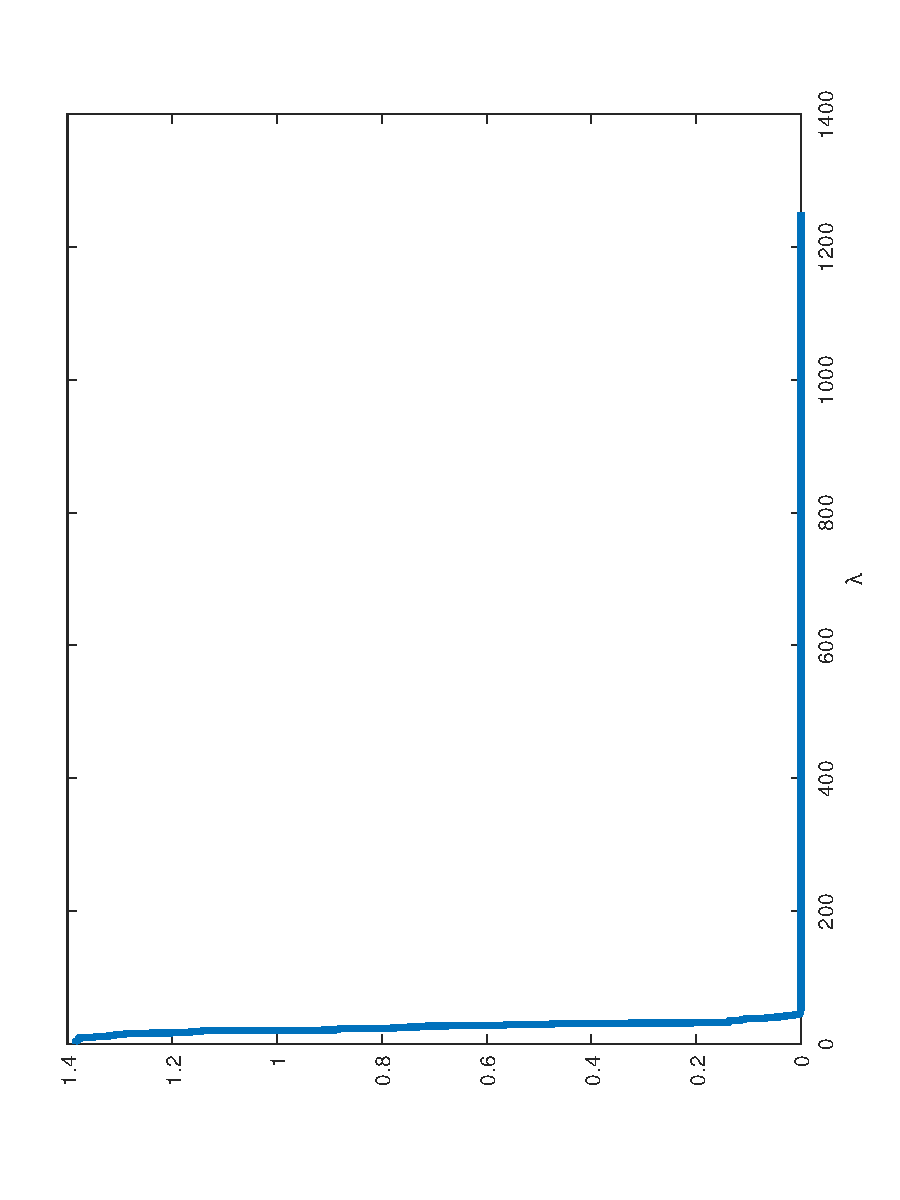
\includegraphics[
        angle=-90,
        origin=c,
        width=\textwidth]{papers/sgwt/images/wavelets/h.pdf}
        \vspace{-45pt}
        \caption{Die Kernelfunktion $h(\lambda)$ eines Kugelgraphen mit 1252 
            Knoten.}
        \label{fig:sgwt:wavelets:sphere:h}
    \end{minipage}
    ~
    \begin{minipage}[t]{0.49\textwidth}
        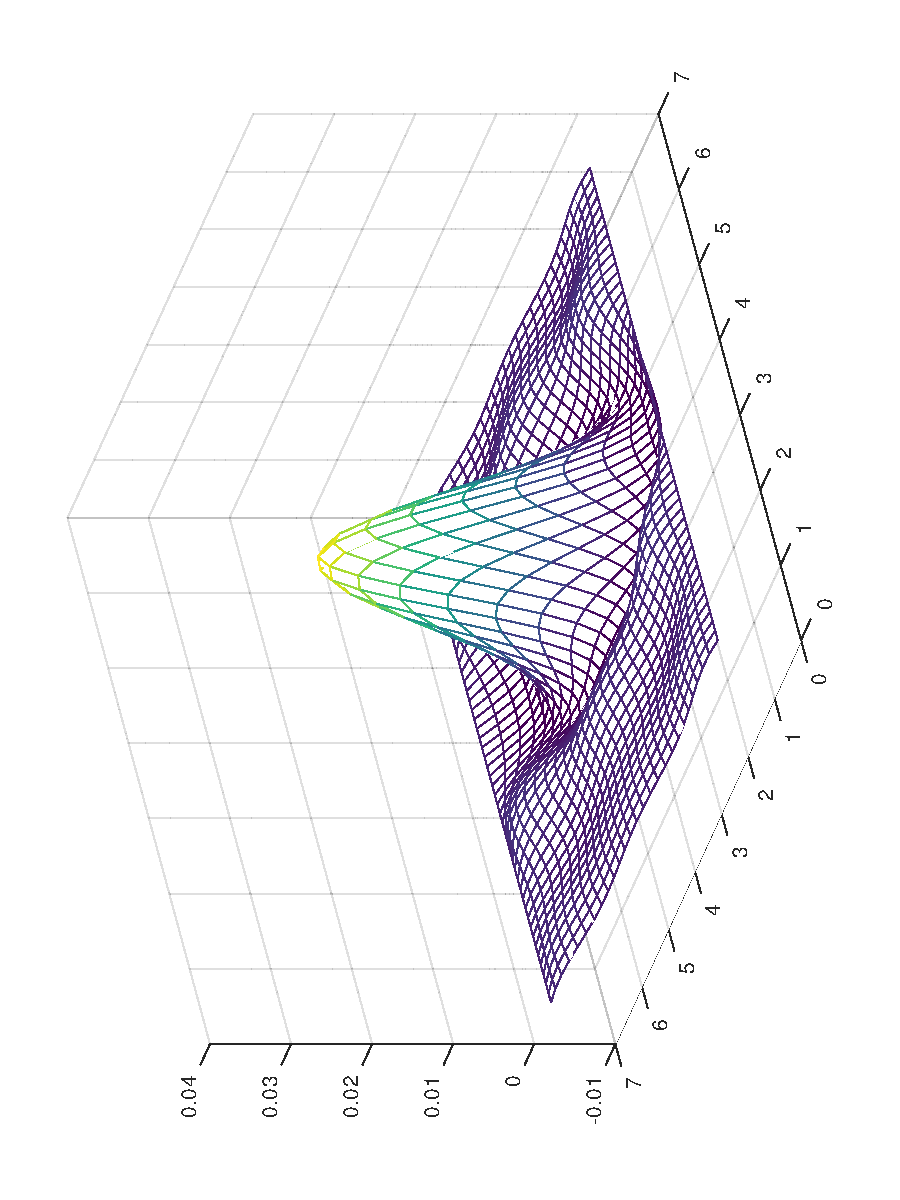
\includegraphics[
        angle=-90,
        origin=c,
        width=\textwidth]{papers/sgwt/images/wavelets/phi_50_25_630_flat.pdf}
        \vspace{-45pt}
        \caption{$\phi(v_{630})$-Wavelet eines Kugelgraphen mit 1252 Knoten.}
        \label{fig:sgwt:wavelets:sphere:phi:flat}
    \end{minipage}
    ~
    \begin{minipage}[t]{\textwidth}
        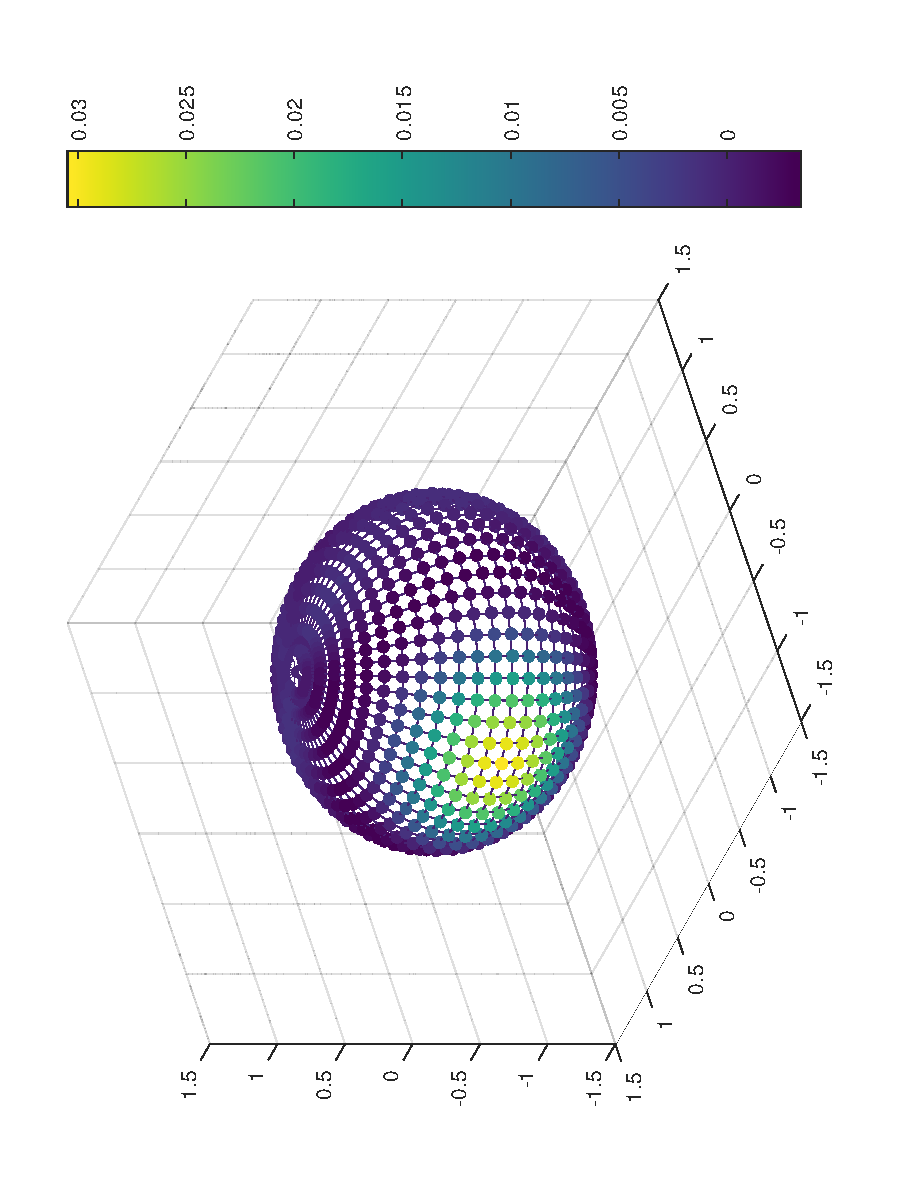
\includegraphics[
        angle=-90,
        origin=c,
        width=\textwidth]{papers/sgwt/images/wavelets/phi_50_25_630.pdf}
        \vspace{-45pt}
        \caption{$\phi(v_{630})$-Wavelet eines Kugelgraphen mit 1252 Knoten.}
        \label{fig:sgwt:wavelets:sphere:phi}
    \end{minipage}
\end{figure}

\subsection{Frames}

Obwohl $t$ ein kontinuierlicher Faktor ist, werden wir uns in der Praxis auf 
$J$ Faktoren, also eine endliche Anzahl $\{t_j\}^J_{j=1}$, beschr\"anken 
m\"ussen. Die Wahl der unterschiedlichen $t_j$ ist frei und kann somit auf den 
jeweiligen Graphen und den Funktionen auf diesem Graphen angepasst werden. 

Mit $h(\lambda)$ und den $J$ skalierten $g(t_j\lambda)$ haben wir dann 
also $J + 1$ Kernelfunktionen f\"ur die Analyse und Synthese zur Verf\"ugung. 
Wir haben es also mit einem also mit einem Frame zu tun, dessen Grenzen durch
\begin{align*}
A &= \min_{\lambda \in \left[0, \lambda_{N-1}\right]} f(\lambda) \\
B &= \max_{\lambda \in \left[0, \lambda_{N-1}\right]} f(\lambda) \\
\text{mit } f(\lambda) &= h(\lambda)^2 + \sum_{j = 1}^{J} g(t_j\lambda)^2
\end{align*}
gegeben sind.

\subsection{\texorpdfstring{$\psi_j$}{psi} und \texorpdfstring{$\phi$}{phi}}
Damit lassen sich nun unsere Wavelets $\psi_j$ und $\phi$ wie folgt konstruieren
\begin{align}
\psi_j = \chi \diag{g(t_j\lambda)} \chi' 
\label{eq:sgwt:psi}
\\
\phi = \chi \diag{h(\lambda)} \chi'.
\label{eq:sgwt:phi}
\end{align}
Zur Veranschaulichung sehen wir hier die Wavelets eines Kreisgraphen 
in~\cref{fig:sgwt:wavelets:ring0,fig:sgwt:wavelets:ring1,fig:sgwt:wavelets:ring2,fig:sgwt:wavelets:ring3,fig:sgwt:wavelets:ring4,fig:sgwt:wavelets:ring5},
 eines Streckengraphen 
in~\cref{fig:sgwt:wavelets:line0,fig:sgwt:wavelets:line1,fig:sgwt:wavelets:line2,fig:sgwt:wavelets:line3,fig:sgwt:wavelets:line4,fig:sgwt:wavelets:line5}
 und eines Kugelgraphen 
in~\cref{fig:sgwt:wavelets:sphere0,fig:sgwt:wavelets:sphere1,fig:sgwt:wavelets:sphere2,fig:sgwt:wavelets:sphere3,fig:sgwt:wavelets:sphere4,fig:sgwt:wavelets:sphere5}.
Gut zu erkennen ist dabei, dass der Kreisgraph die wohl beste Approximation der 
bisherigen Wavelettheorie ist. Beim Streckengraph fehlt die Periodisierung, die 
wir durch die Verbindungskante des Start- und Endknoten beim Kreisgraphen 
erreicht haben. Auch beim Kugelgraphen wird klar, dass die Pole, aufgrund ihres 
viel gr\"osseren Grades, deutlich st\"arker gewichtet werden und es daher zu 
einer Verzerrung der Wavelets in Richtung der Pole kommt.

\begin{figure}
    \centering
    \begin{minipage}[t]{0.49\textwidth}
        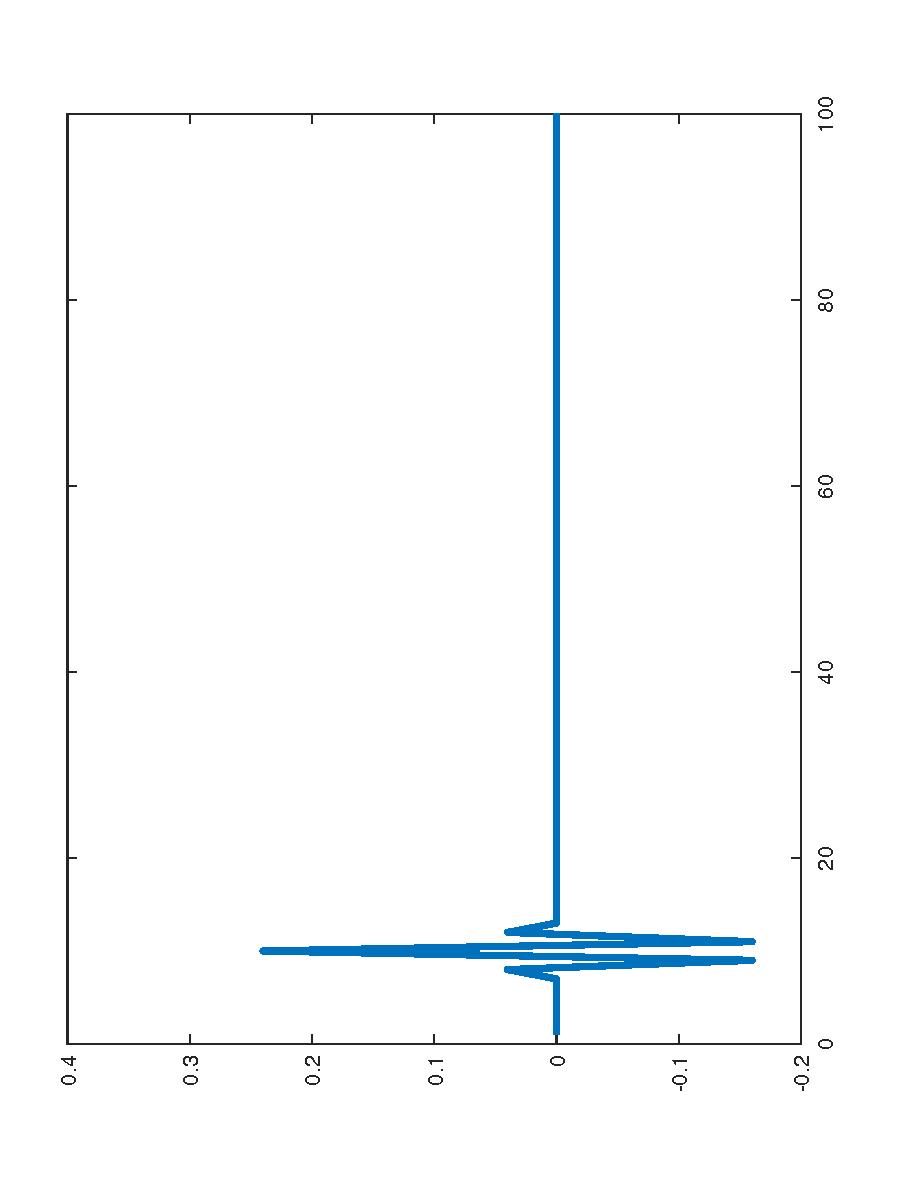
\includegraphics[
        angle=-90,
        origin=c,
        width=\textwidth]{papers/sgwt/images/wavelets-psi-1-10.pdf}
        \vspace{-45pt}
        \caption{$\psi_1(v_{10})$-Wavelets eines Kreisgraphen mit 100 Knoten.}
        \label{fig:sgwt:wavelets:ring0}
    \end{minipage}
    ~
    \begin{minipage}[t]{0.49\textwidth}
        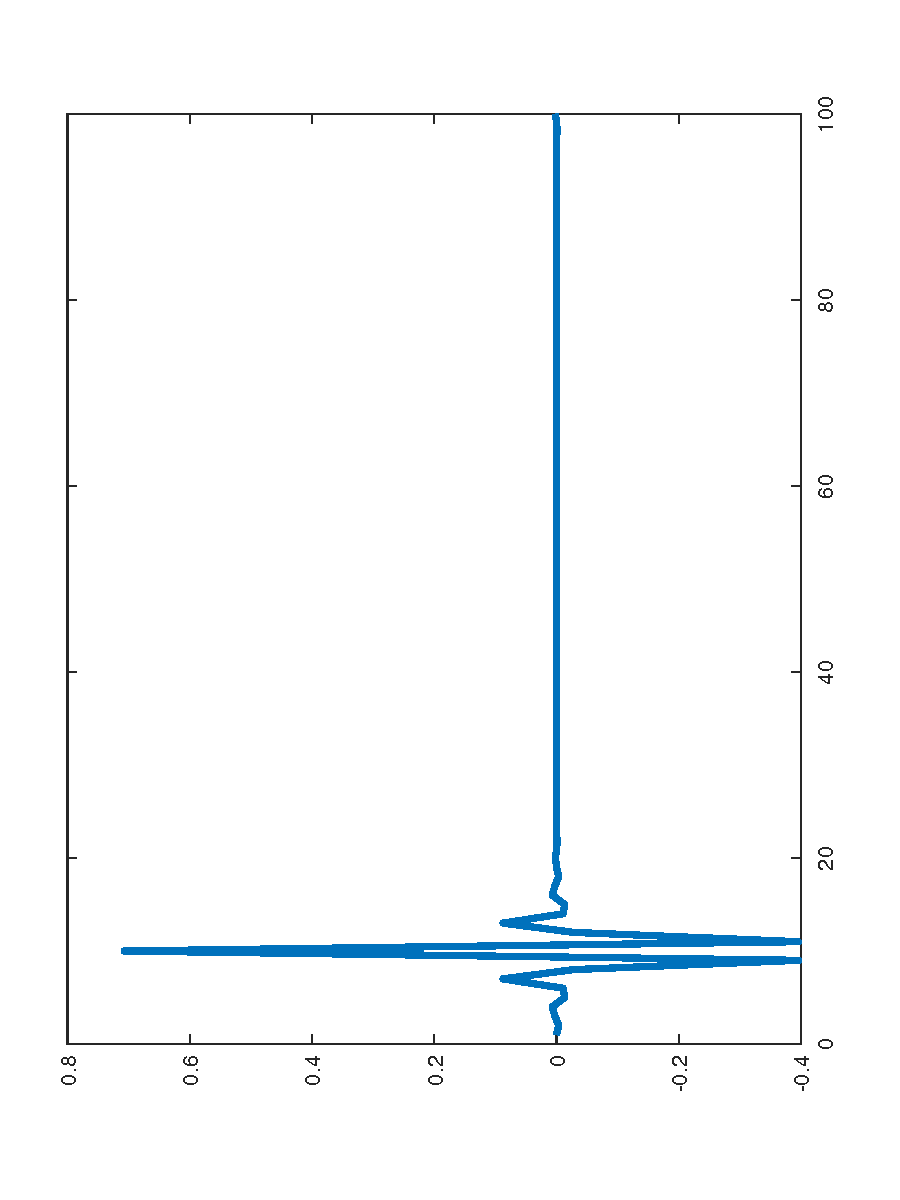
\includegraphics[
        angle=-90,
        origin=c,
        width=\textwidth]{papers/sgwt/images/wavelets-psi-2-10.pdf}
        \vspace{-45pt}
        \caption{$\psi_2(v_{10})$-Wavelets eines Kreisgraphen mit 100 Knoten.}
        \label{fig:sgwt:wavelets:ring1}
    \end{minipage}
    ~
    \begin{minipage}[t]{0.49\textwidth}
        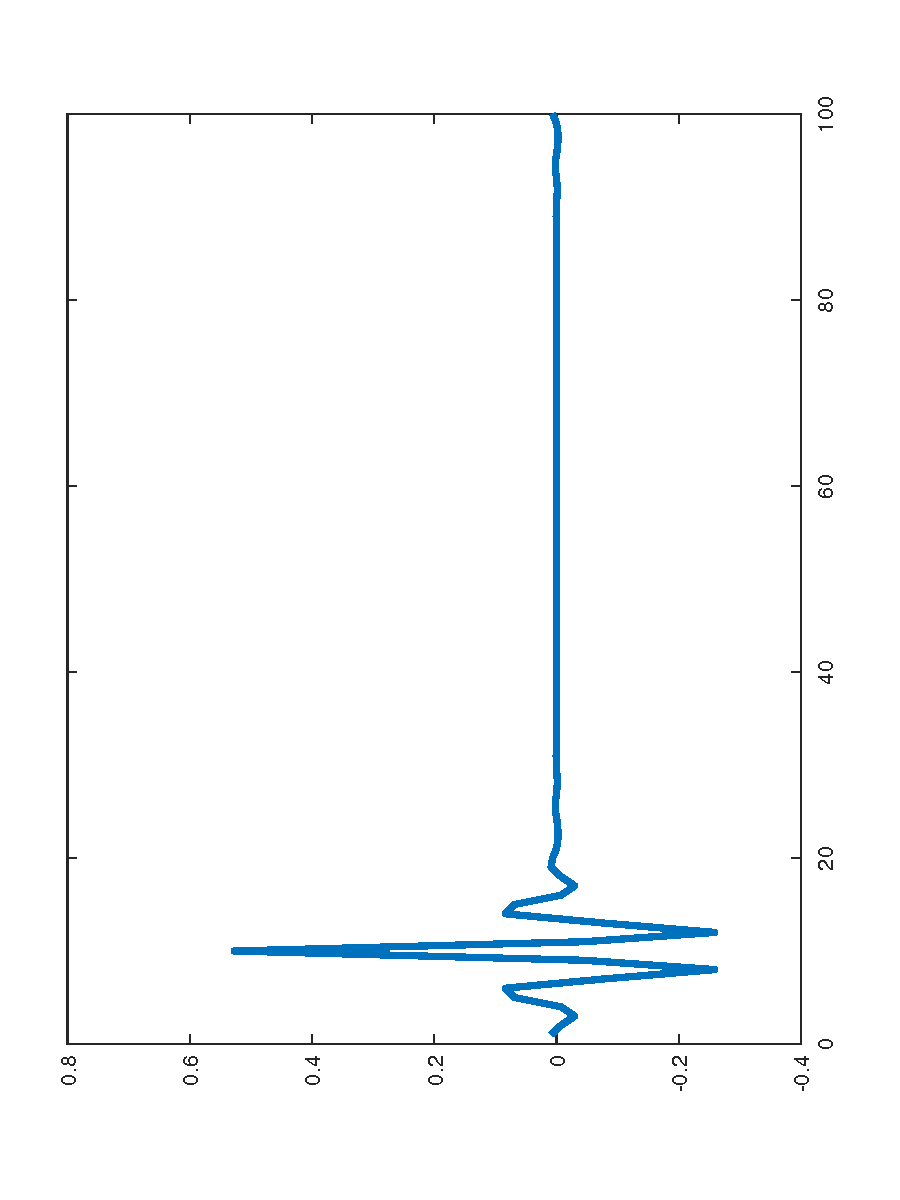
\includegraphics[
        angle=-90,
        origin=c,
        width=\textwidth]{papers/sgwt/images/wavelets-psi-3-10.pdf}
        \vspace{-45pt}
        \caption{$\psi_3(v_{10})$-Wavelets eines Kreisgraphen mit 100 Knoten.}
        \label{fig:sgwt:wavelets:ring2}
    \end{minipage}
    ~
    \begin{minipage}[t]{0.49\textwidth}
        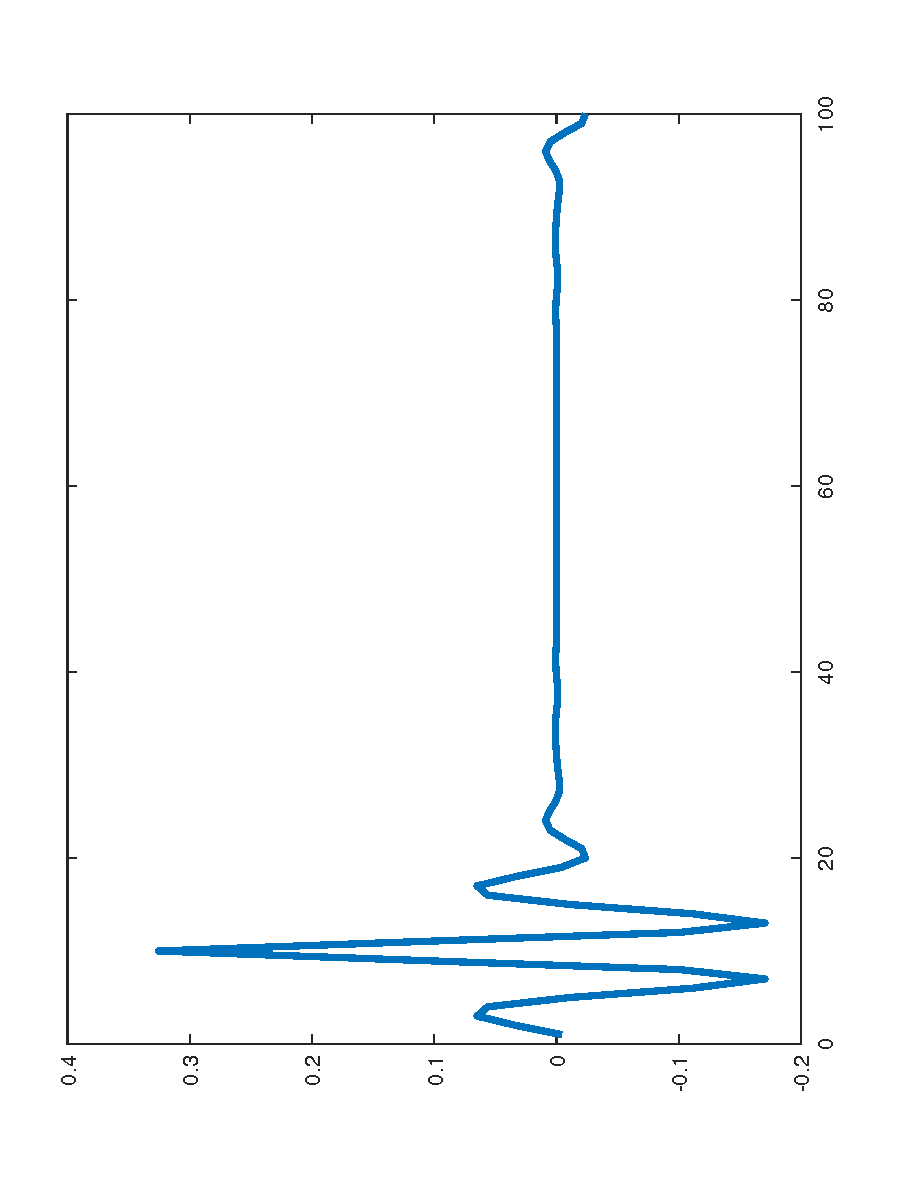
\includegraphics[
        angle=-90,
        origin=c,
        width=\textwidth]{papers/sgwt/images/wavelets-psi-4-10.pdf}
        \vspace{-45pt}
        \caption{$\psi_4(v_{10})$-Wavelets eines Kreisgraphen mit 100 Knoten.}
        \label{fig:sgwt:wavelets:ring3}
    \end{minipage}
    ~
    \begin{minipage}[t]{0.49\textwidth}
        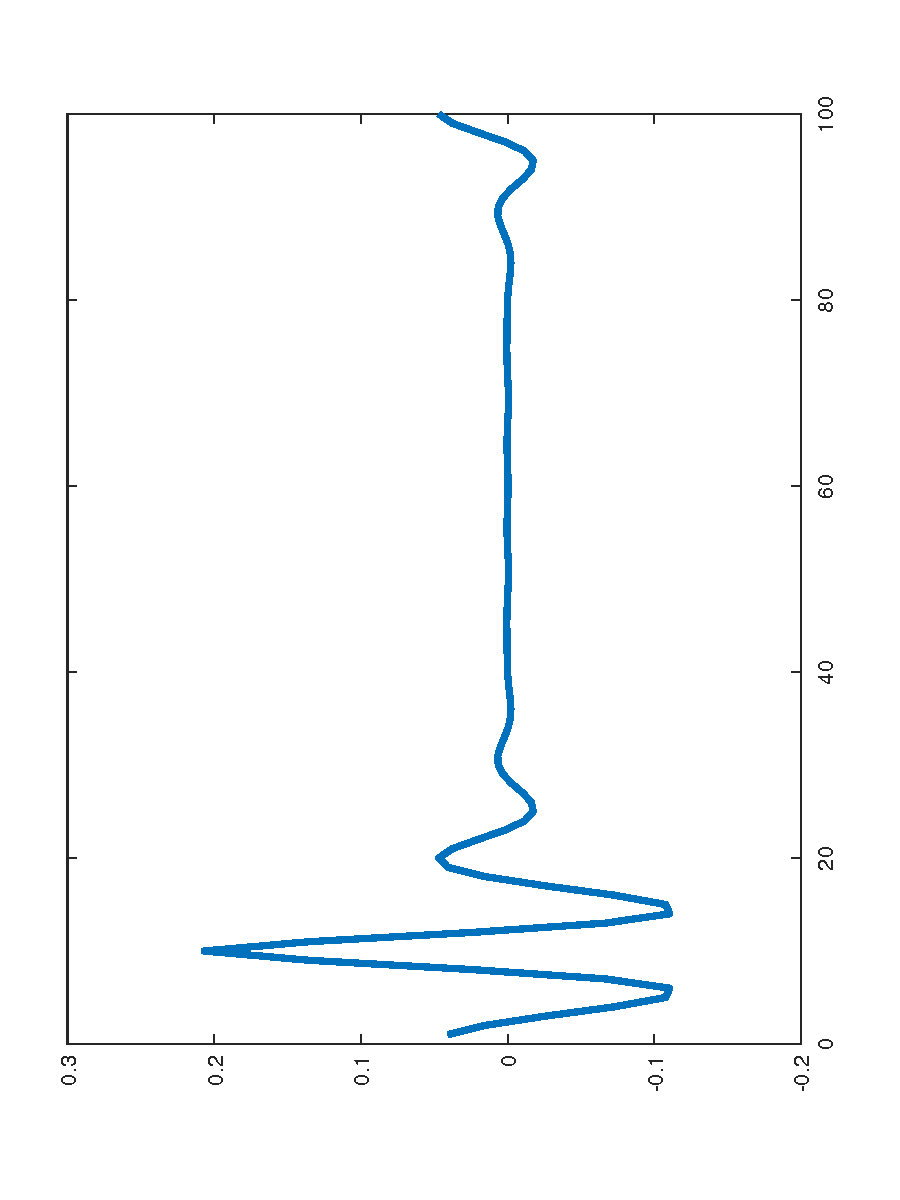
\includegraphics[
        angle=-90,
        origin=c,
        width=\textwidth]{papers/sgwt/images/wavelets-psi-5-10.pdf}
        \vspace{-45pt}
        \caption{$\psi_5(v_{10})$-Wavelets eines Kreisgraphen mit 100 Knoten.}
        \label{fig:sgwt:wavelets:ring4}
    \end{minipage}
    ~
    \begin{minipage}[t]{0.49\textwidth}
        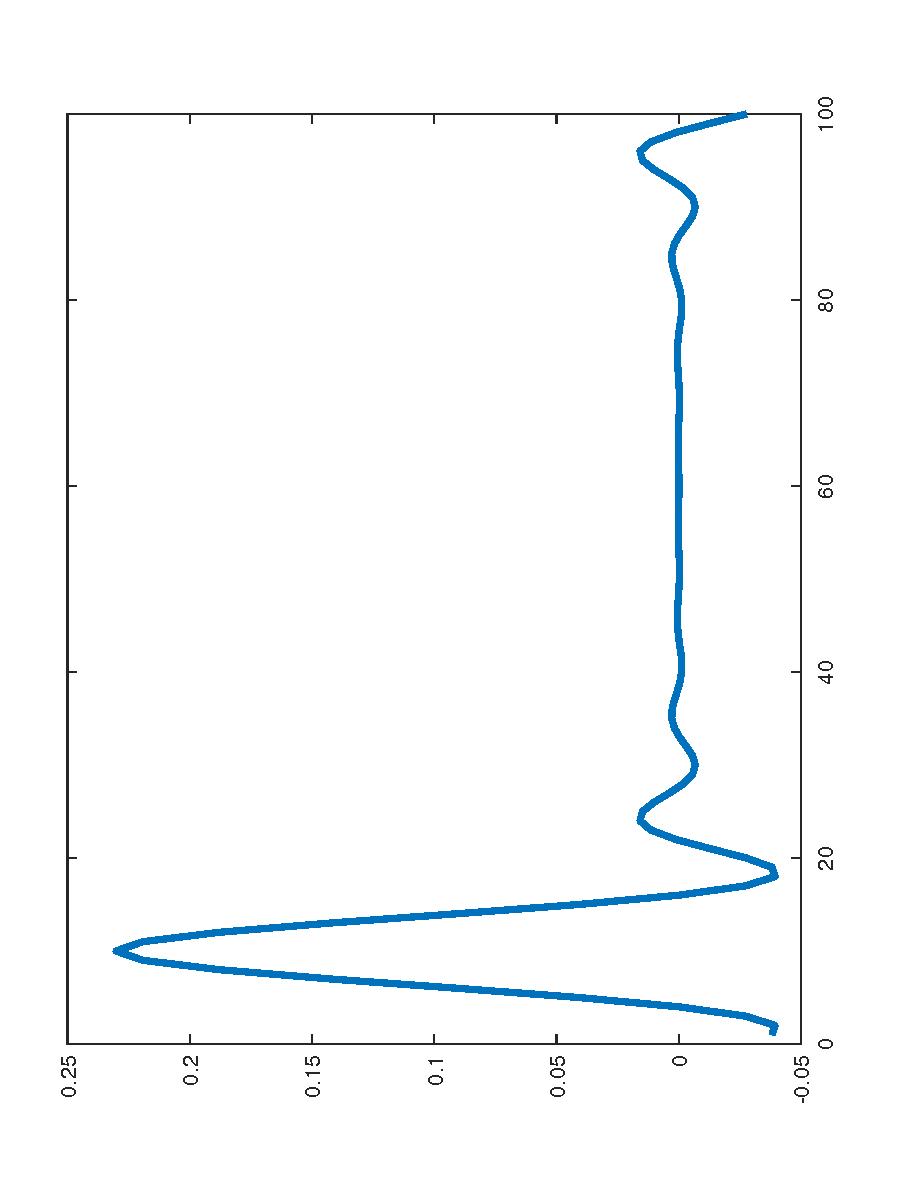
\includegraphics[
        angle=-90,
        origin=c,
        width=\textwidth]{papers/sgwt/images/wavelets-phi-10.pdf}
        \vspace{-45pt}
        \caption{$\phi(v_{10})$-Wavelets eines Kreisgraphen mit 100 Knoten.}
        \label{fig:sgwt:wavelets:ring5}
    \end{minipage}
\end{figure}

\begin{figure}
    \centering
    \begin{minipage}[t]{0.49\textwidth}
        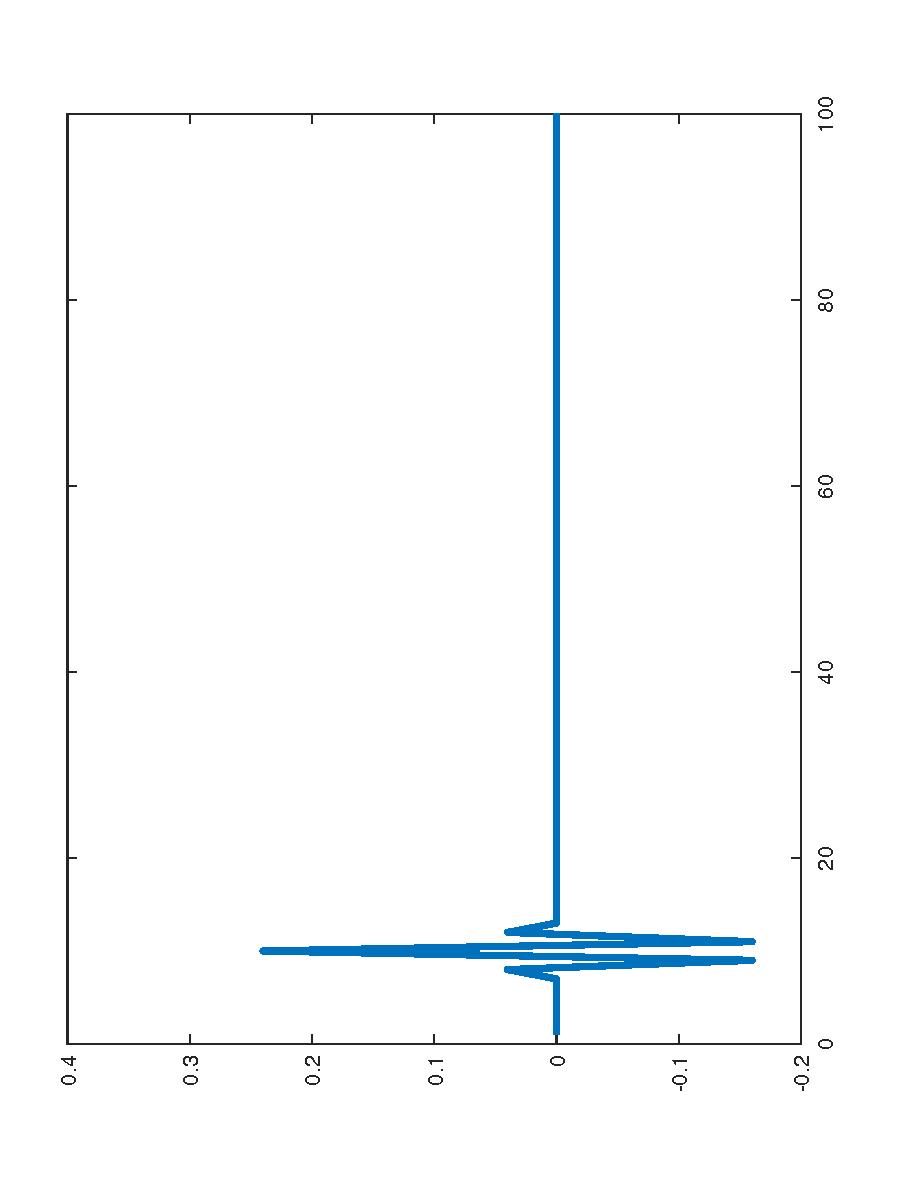
\includegraphics[
        angle=-90,
        origin=c,
        width=\textwidth]{papers/sgwt/images/wavelets-psi-line-1-10.pdf}
        \vspace{-45pt}
        \caption{$\psi_1(v_{10})$-Wavelets eines Streckengraphen mit 100 
        Knoten.}
        \label{fig:sgwt:wavelets:line0}
    \end{minipage}
    ~
    \begin{minipage}[t]{0.49\textwidth}
        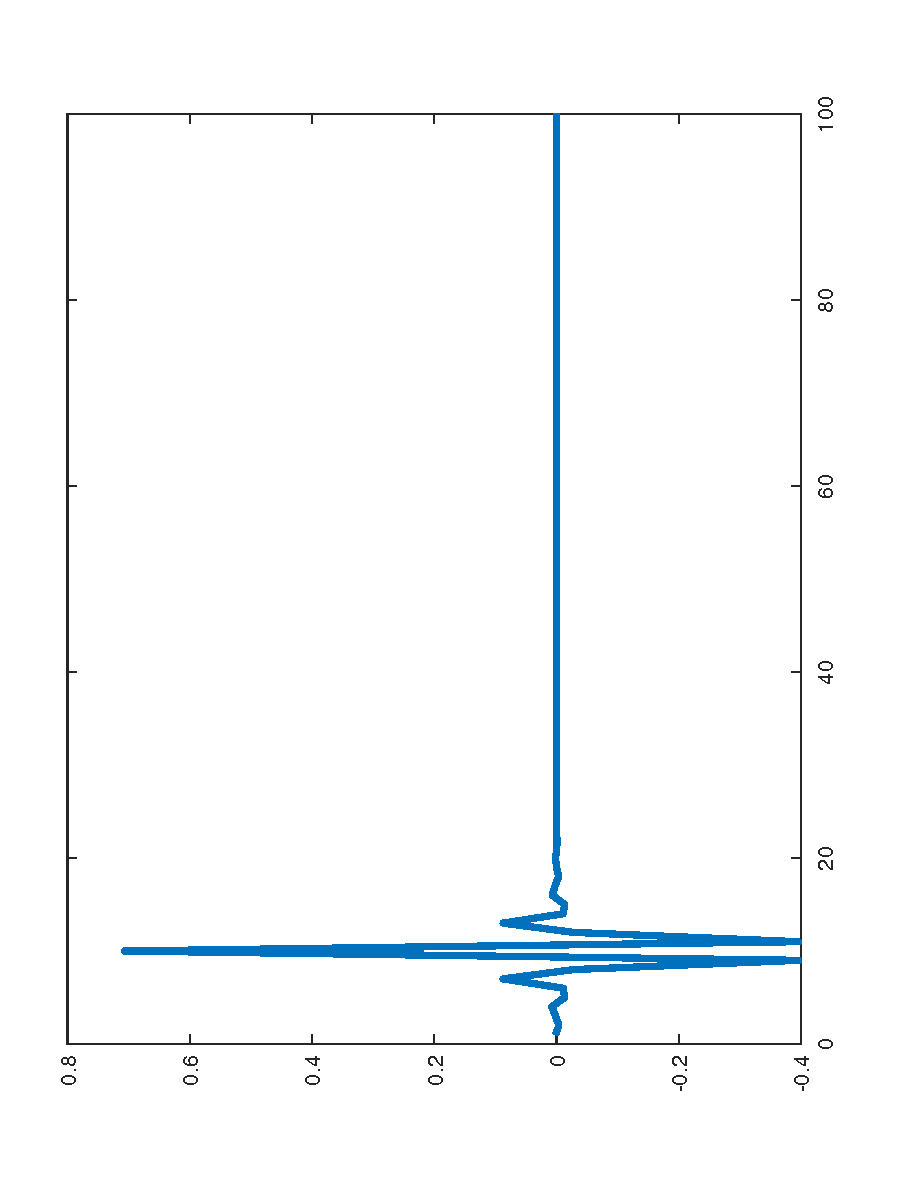
\includegraphics[
        angle=-90,
        origin=c,
        width=\textwidth]{papers/sgwt/images/wavelets-psi-line-2-10.pdf}
        \vspace{-45pt}
        \caption{$\psi_2(v_{10})$-Wavelets eines Streckengraphen mit 100 
        Knoten.}
        \label{fig:sgwt:wavelets:line1}
    \end{minipage}
    ~
    \begin{minipage}[t]{0.49\textwidth}
        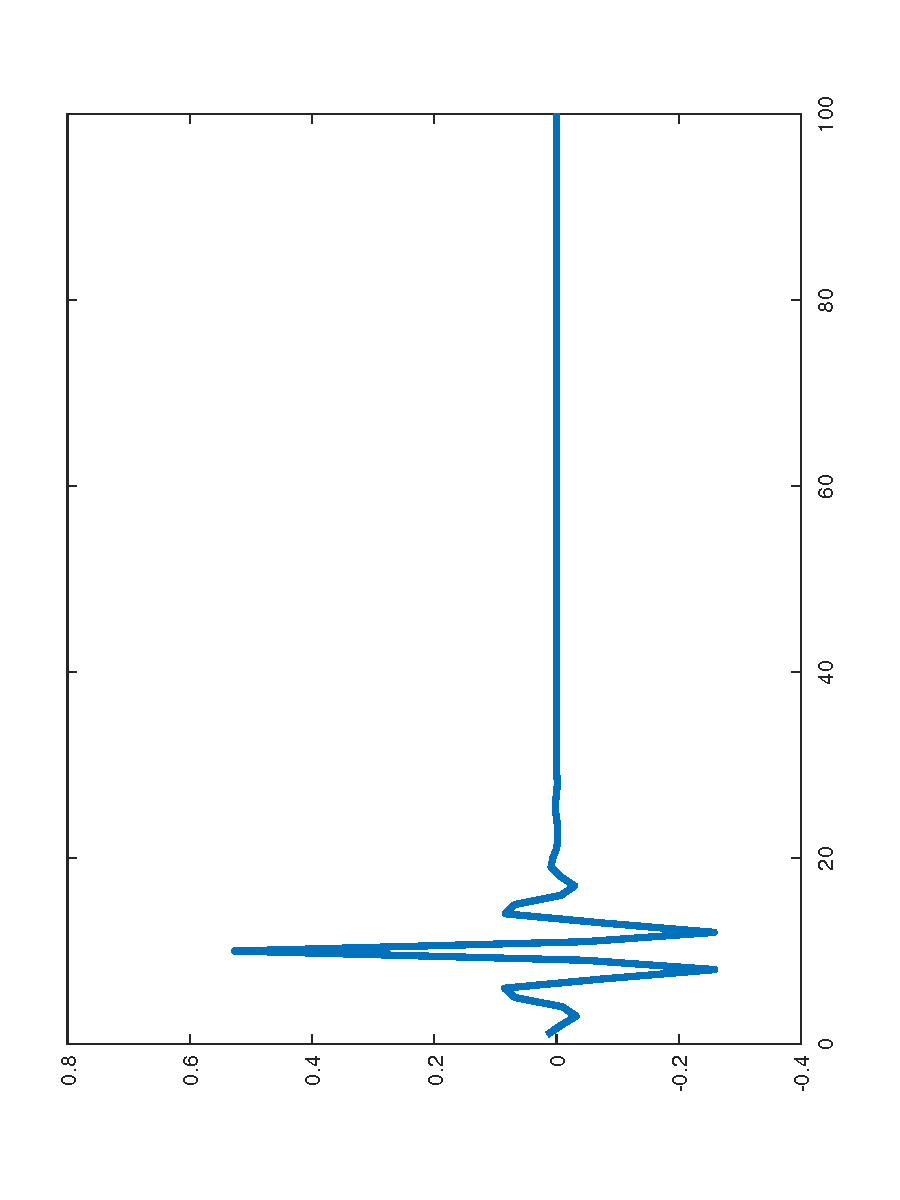
\includegraphics[
        angle=-90,
        origin=c,
        width=\textwidth]{papers/sgwt/images/wavelets-psi-line-3-10.pdf}
        \vspace{-45pt}
        \caption{$\psi_3(v_{10})$-Wavelets eines Streckengraphen mit 100 
        Knoten.}
        \label{fig:sgwt:wavelets:line2}
    \end{minipage}
    ~
    \begin{minipage}[t]{0.49\textwidth}
        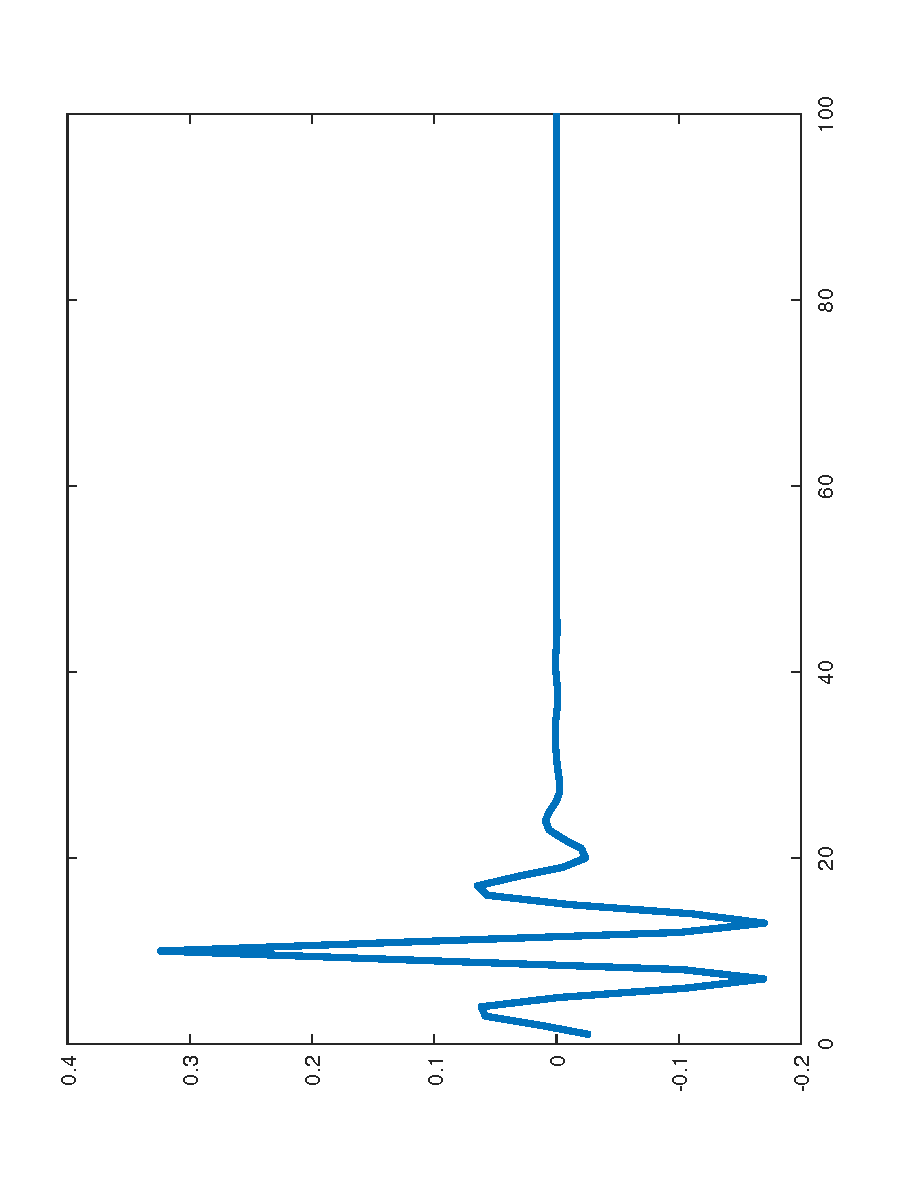
\includegraphics[
        angle=-90,
        origin=c,
        width=\textwidth]{papers/sgwt/images/wavelets-psi-line-4-10.pdf}
        \vspace{-45pt}
        \caption{$\psi_4(v_{10})$-Wavelets eines Streckengraphen mit 100 
        Knoten.}
        \label{fig:sgwt:wavelets:line3}
    \end{minipage}
    ~
    \begin{minipage}[t]{0.49\textwidth}
        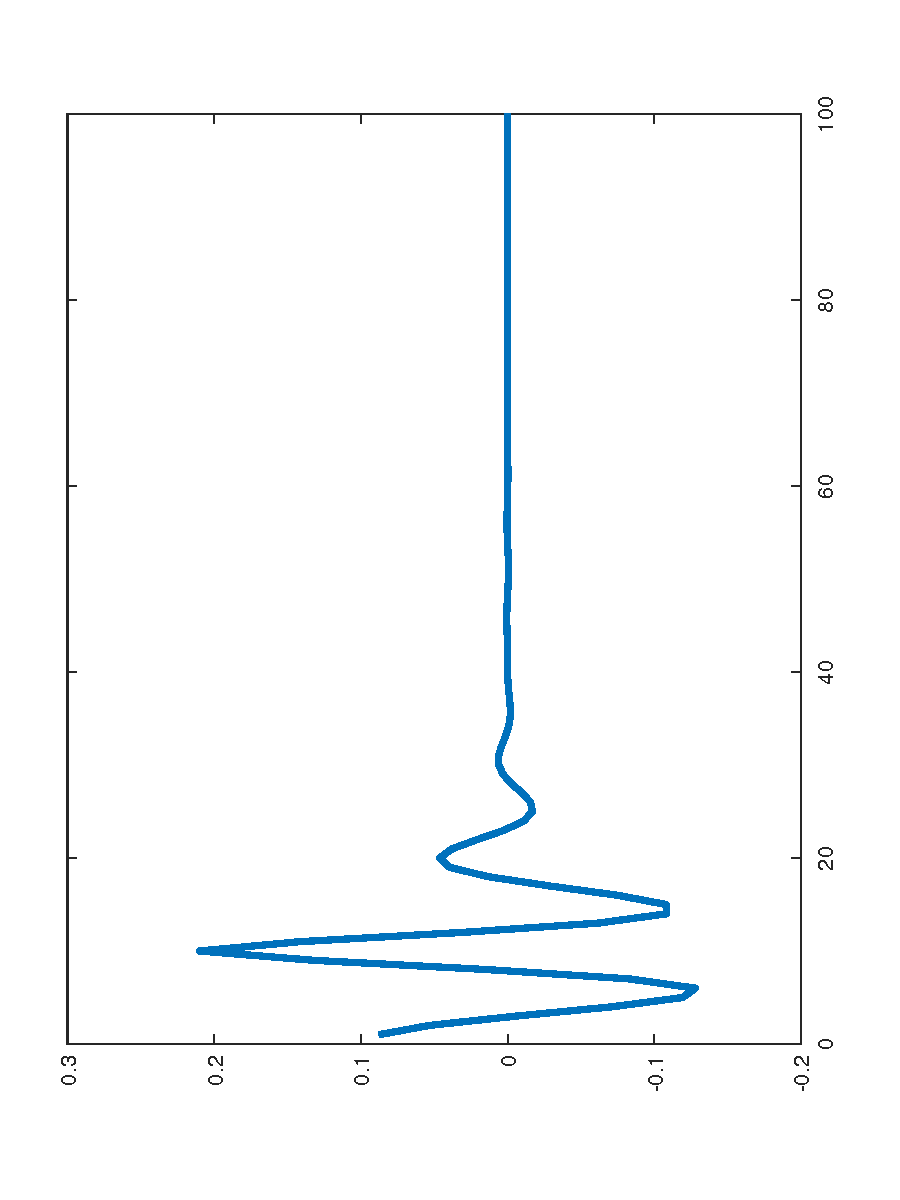
\includegraphics[
        angle=-90,
        origin=c,
        width=\textwidth]{papers/sgwt/images/wavelets-psi-line-5-10.pdf}
        \vspace{-45pt}
        \caption{$\psi_5(v_{10})$-Wavelets eines Streckengraphen mit 100 
        Knoten.}
        \label{fig:sgwt:wavelets:line4}
    \end{minipage}
    ~
    \begin{minipage}[t]{0.49\textwidth}
        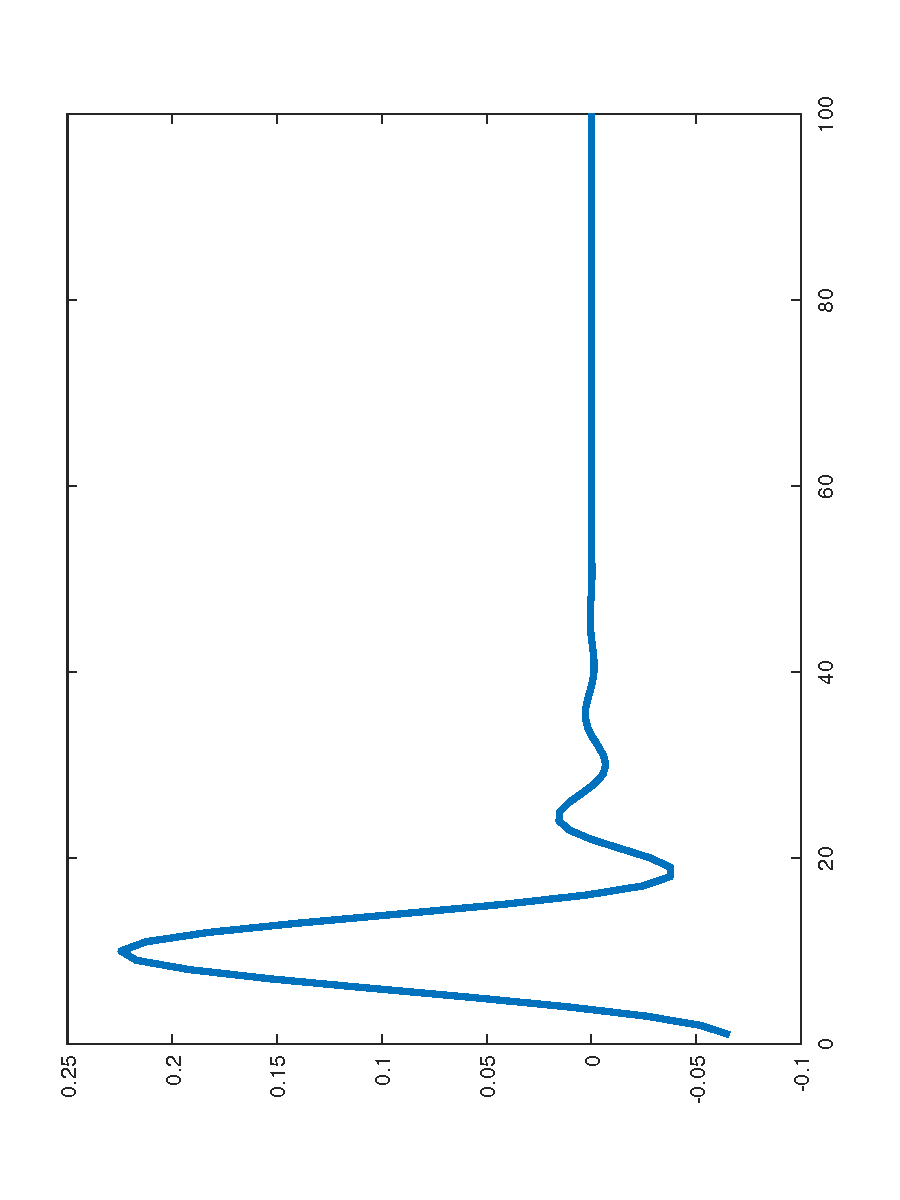
\includegraphics[
        angle=-90,
        origin=c,
        width=\textwidth]{papers/sgwt/images/wavelets-phi-line-10.pdf}
        \vspace{-45pt}
        \caption{$\phi(v_{10})$-Wavelets eines Streckengraphen mit 100 Knoten.}
        \label{fig:sgwt:wavelets:line5}
    \end{minipage}
\end{figure}

Die Wavelets k\"onnen wir dann wieder ein die $N(J+1)\text{x}N$-Matrix $T$ 
packen um dann die Wavelet Koeffizienten wie folgt zu berechnen
\begin{equation}
\hat{f} = T f.
\label{eq:sgwt:hatf}
\end{equation}

\subsection{SGWT Analyse und Synthese}

Um nun eine Funktion $f(v)$ auf einem Graphen $G$ zu analysieren gehen wir 
also wie folgt vor:
\begin{itemize}
    \item[1.] Generierung der \laplaceL{} Matrix aus dem Graphen $G$.
    \item[2.] Berechnung der Eigenwerte $\lambda$ und Eigenvektoren $\chi$.
    \item[3.] Berechnung der $\psi_j$ und $\phi$ Wavelets 
    mit~\cref{eq:sgwt:psi,eq:sgwt:phi}.
    \item[4.] Berechnung der Wavelet Koeffizienten $\hat{f}$ 
    mit~\cref{eq:sgwt:hatf}.
\end{itemize}

F\"ur die Synthese nehmen wir als Eingabe die bei der Analyse berechnet und 
danach m\"oglicherweise bearbeiteten $\hat{f}$. Zus\"atzlich brauchen wir die 
$T$ Matrix, mit deren Inversen wir wieder die Funktion
\begin{equation}
f = T^{-1} \hat{f}
\end{equation}
synthetisieren. Da diese Matrix aber nicht mehr quadratisch ist, kann sie nicht 
mehr so einfach invertiert werden. Wir nehmen uns daher das Pseudoinverse $L = 
(T^*T)^{-1}T^*$ zur Hilfe und erhalten
\begin{equation}
f = L \hat{f} = (T^*T)^{-1}T^* \hat{f}.
\end{equation}
